\chapter*{Anhang}\addcontentsline{toc}{chapter}{Anhang} 
\markboth{\MakeMarkcase{Anhang}}{\MakeMarkcase{Anhang}}
\label{cha:Anhang}
\section*{Der Fragebogen}
\label{Anh:Fragebogen}
%(wie er aussieht und die Codes)\\
%\par
%\begingroup
%\leftskip4em
%\rightskip\leftskip
%\textbf{Herzlich willkommen!} Diese Untersuchung findet im Rahmen einer Doktorarbeit in der \textbf{Sprachwissenschaft des Deutschen} statt. Vielen Dank, dass Sie sich die Zeit nehmen, den Fragebogen zu bearbeiten.
%Die Bearbeitung des Fragebogens wird \textbf{ungefähr 15-20 Minuten} dauern. Alle Angaben erfolgen anonym und dienen rein wissenschaftlichen Zwecken. 
%Wir beginnen zunächst mit ein paar Fragen zu Ihrer persönlichen Einstellung zum Thema Grammatik.  
%\par
%\endgroup
\begin{figure}
\centering

\includegraphics[width=.7\textwidth]{Fb1.png}
\end{figure}
\begin{figure}
\centering
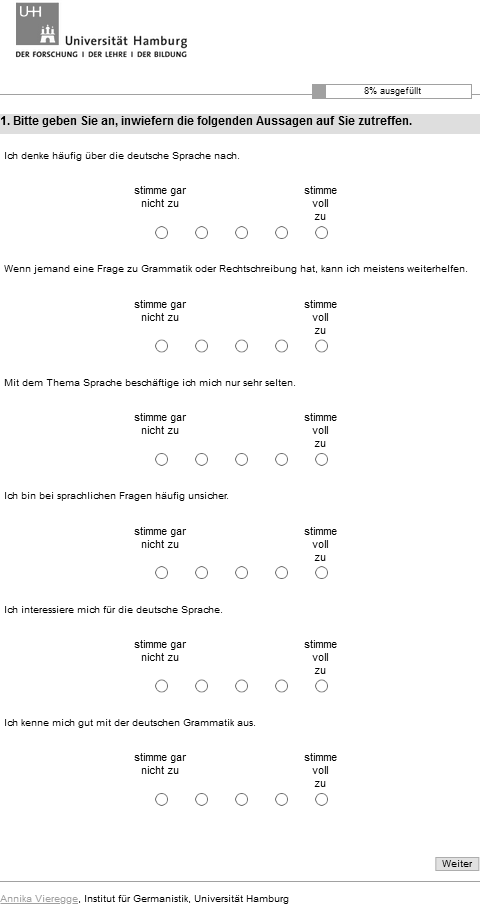
\includegraphics[width=.7\textwidth]{Fb2.png}
\end{figure}
\begin{figure}
\centering
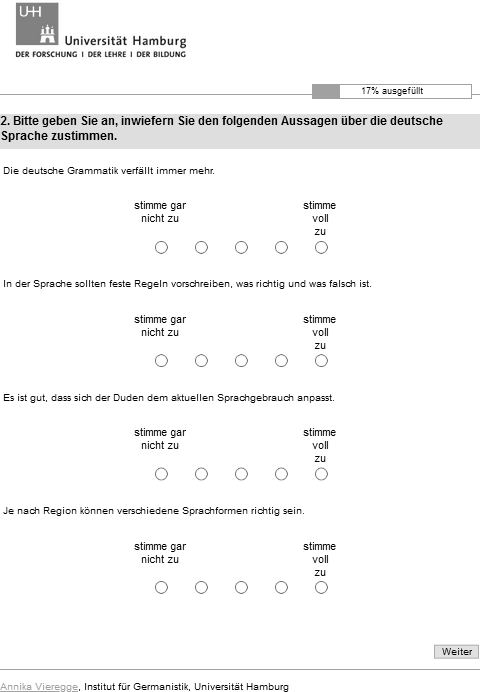
\includegraphics[width=.7\textwidth]{Fb3.png}
\end{figure}
\newpage
\begin{figure}
\centering
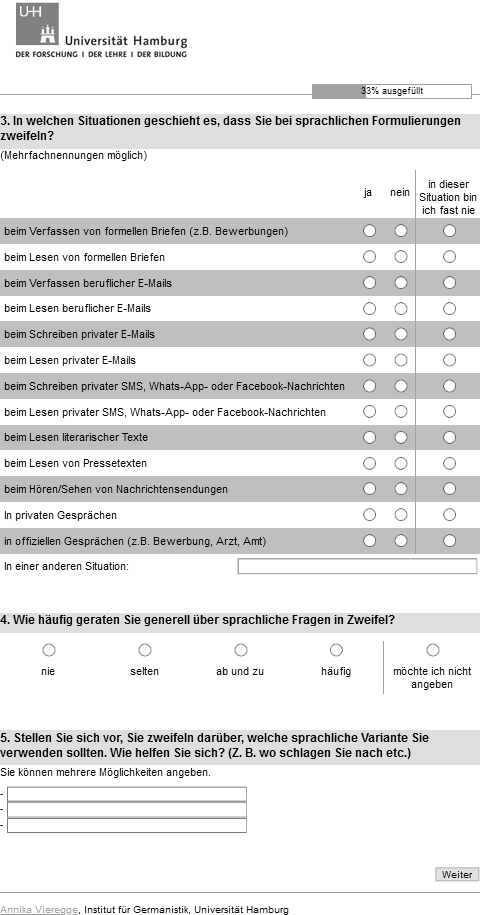
\includegraphics[width=.7\textwidth]{Fb4.png}
\end{figure}
\begin{figure}
\centering
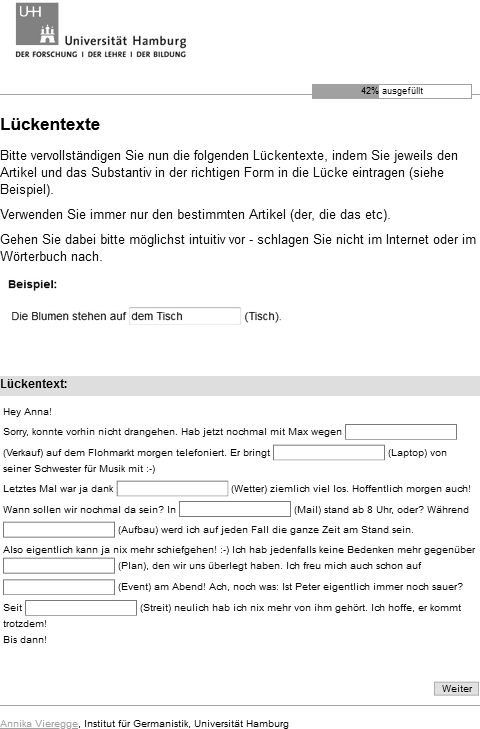
\includegraphics[width=.7\textwidth]{Fb5.png}
\end{figure}
\newpage
\begin{figure}
\centering
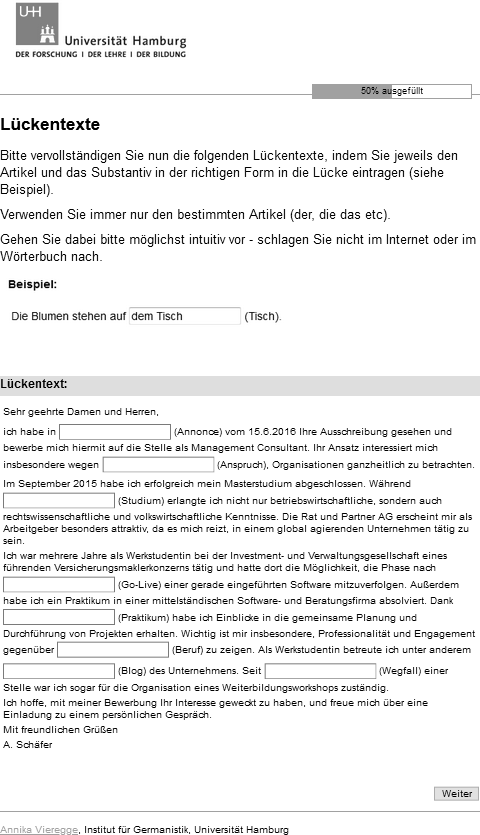
\includegraphics[width=.7\textwidth]{Fb6.png}
\end{figure}
\begin{figure}
\centering
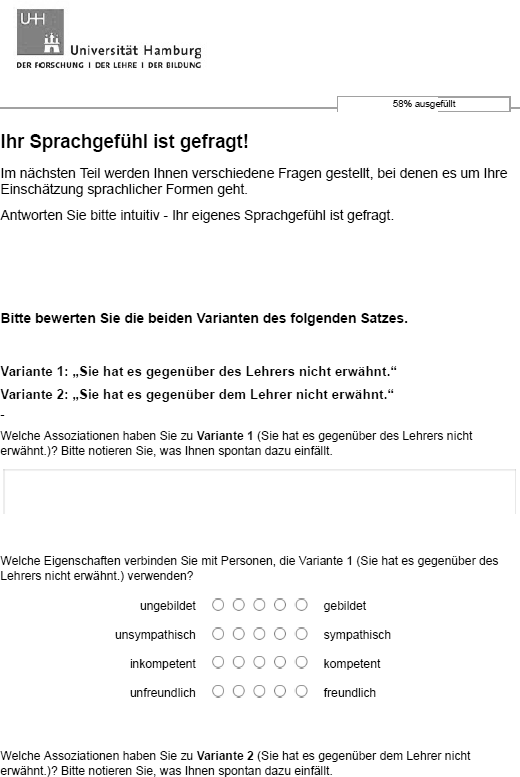
\includegraphics[width=.7\textwidth]{Fb7a.png}
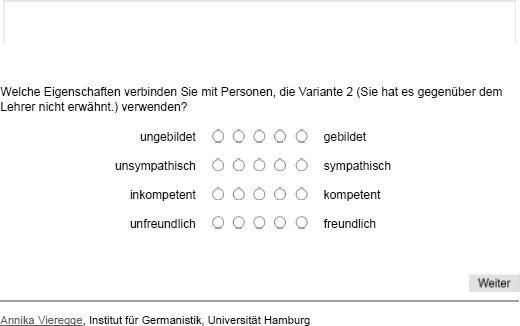
\includegraphics[width=.7\textwidth]{Fb7b.png}
\end{figure}
\begin{figure}
\centering
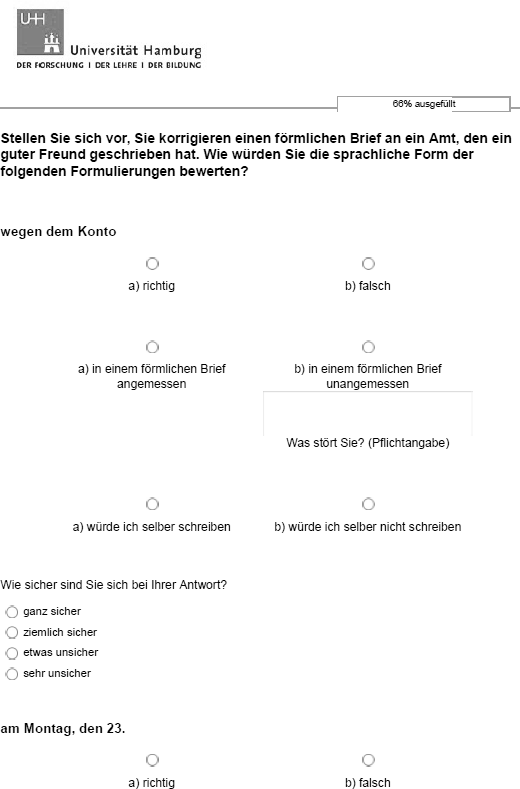
\includegraphics[width=.7\textwidth]{Fb8a.png}
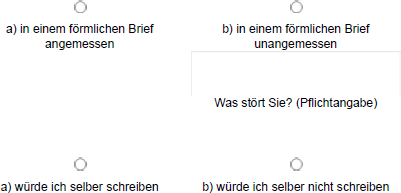
\includegraphics[width=.7\textwidth]{Fb8b.png}
\end{figure}
\begin{figure}
\centering
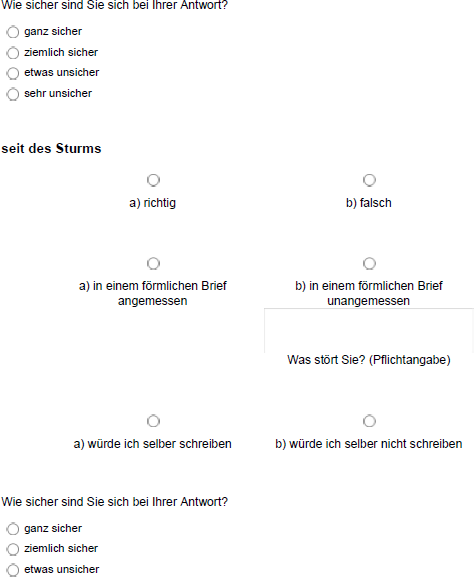
\includegraphics[width=.7\textwidth]{Fb8c.png}
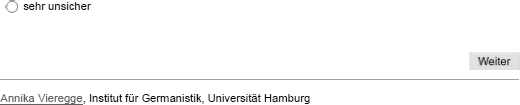
\includegraphics[width=.7\textwidth]{Fb8d.png}
\end{figure}
\begin{figure}
\centering
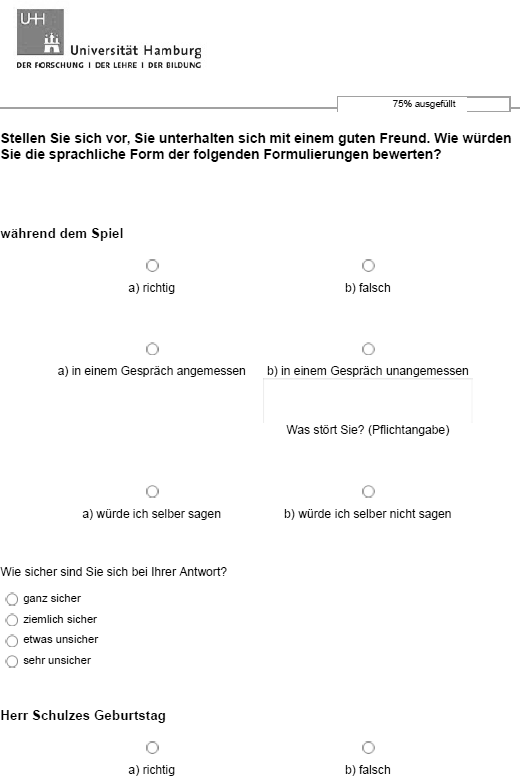
\includegraphics[width=.7\textwidth]{Fb9a.png}
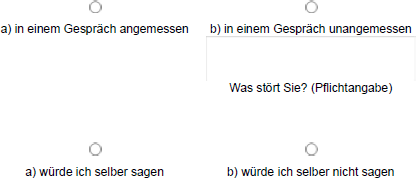
\includegraphics[width=.7\textwidth]{Fb9b.png}
\end{figure}
\begin{figure}
\centering
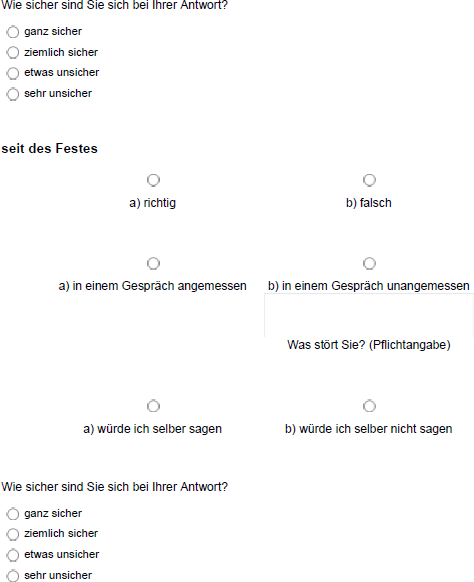
\includegraphics[width=.7\textwidth]{Fb9c.png}
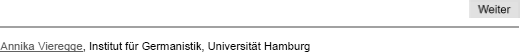
\includegraphics[width=.7\textwidth]{Fb9d.png}
\end{figure}
\begin{figure}
\centering
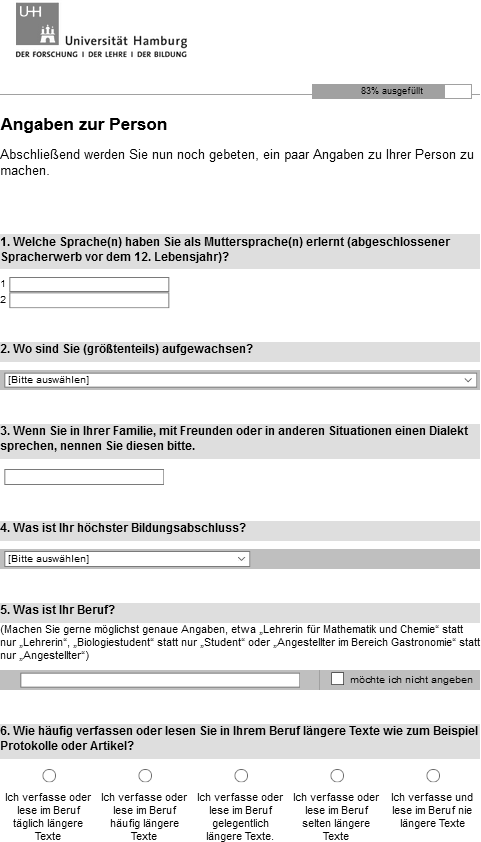
\includegraphics[width=.7\textwidth]{Fb10a.png}
\end{figure}
\begin{figure}
\centering
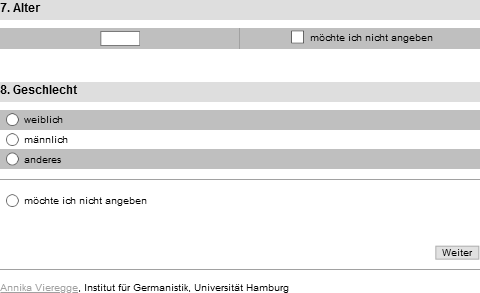
\includegraphics[width=.7\textwidth]{Fb10b.png}
\end{figure}
\begin{figure}
\centering
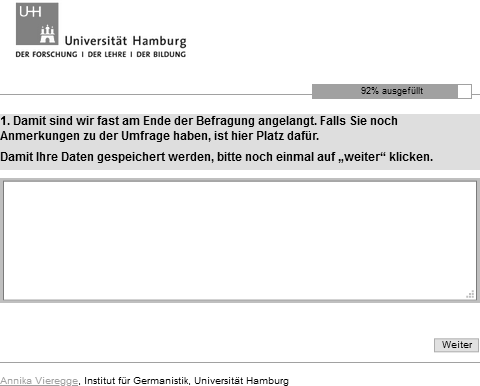
\includegraphics[width=.7\textwidth]{Fb11.png}
\end{figure}
\begin{figure}
\centering

\includegraphics[width=.7\textwidth]{Fb12.png}
\end{figure}
\section*{Soziodemografische Daten der Befragten}
\label{Anh:SoziodemografischeDaten}
\begin{table}
\centering
\begin{tabular}{lrr}
\textbf{Gender} & \multicolumn{1}{l}{\textbf{abs. Häufigkeit}} & \multicolumn{1}{l}{\textbf{Prozentangaben}} \\ \hline
weiblich & 234 & 58,94 \% \\ %\hline
männlich & 155 & 39,04 \% \\ %\hline
anderes & 1 & 0,25 \% \\ %\hline
NA (möchte ich nicht angeben) & 7 & 1,76 \% \\ %\hline
gesamt & 397 & 100,00 \%
\end{tabular}
\caption{Genderangaben der Befragten}
\label{table:GenderAnh}
\end{table}

\begin{table}
\centering
\begin{tabular}{lrr}
\textbf{Altersgruppe} & \multicolumn{1}{l}{\textbf{abs. Häufigkeit}} & \multicolumn{1}{l}{\textbf{Prozentangaben}} \\ \hline
18-25 & 104 & 26,20 \% \\ %\hline
26-35 & 144 & 36,27 \% \\ %\hline
36-60 & 82 & 20,65 \% \\ %\hline
61-85 & 47 & 11,84 \% \\ %\hline
NA & 20 & 5,04 \% \\ %\hline
gesamt & 397 & 100,00 \%
\end{tabular}
\caption{Altersangaben der Befragten}
\label{table:AltersgruppenAnh}
\end{table}

\begin{table}
\centering
\begin{tabular}{lrr}
\textbf{Höchster Abschluss} & \multicolumn{1}{l}{\textbf{abs. Häufigkeit}} & \multicolumn{1}{l}{\textbf{Prozentangaben}} \\ \hline
kein Abitur & 37 & 9,32 \%\\ %\hline
Abitur/Fachabitur & 92 & 23,17 \%\\ %\hline
Hochschulabschluss & 234 & 58,94 \%\\ %\hline
Promotion oder Habilitation & 29 & 7,30 \%\\ %\hline
anderer Abschluss & 5 & 1,26 \%\\ %\hline
gesamt & 397 & 100 \%
\end{tabular}
\caption{Angaben der Befragten zum höchsten Bildungsabschluss}
\label{table:BildungsstandAnh}
\end{table}

\begin{table}
\centering
\begin{tabular}{lrr}
\textbf{Herkunft} & \multicolumn{1}{l}{\textbf{abs. Häufigkeit}} & \multicolumn{1}{l}{\textbf{Prozentangaben}} \\ \hline
\begin{tabular}[c]{@{}l@{}}\textbf{Norddeutschland}\\ \begin{small}(Schleswig-Holstein, Niedersachsen,\end{small}\\ \begin{small}Bremen, Hamburg)\end{small}\end{tabular} & 172 & 43,32 \% \\ \hline
\begin{tabular}[c]{@{}l@{}}\textbf{Süddeutschland}\\\begin{small}(Bayern, Baden-Württemberg)\end{small}\end{tabular} & 100 & 25,19 \% \\ \hline
\begin{tabular}[c]{@{}l@{}}\textbf{West-/Südwestdeutschland}\\ \begin{small}(Nordrhein-Westfalen, Hessen,\end{small}\\ \begin{small}Rheinland-Pfalz, Saarland)\end{small}\end{tabular} & 99 & 24,94 \% \\ \hline
\begin{tabular}[c]{@{}l@{}}\textbf{Ost-/Nordostdeutschland}\\ \begin{small}(Brandenburg, Mecklenburg-Vorpommern,\end{small}\\ \begin{small}Sachsen, Thüringen, Sachsen-Anhalt, Berlin)\end{small}\end{tabular} & 26 & 6,55 \% \\ \hline
gesamt & 397 & 100,00 \% 
\end{tabular}
\caption{Herkunftsangaben der Befragten}
\label{table:HerkunftAnh}
\end{table}

\begin{table}
\centering
\begin{tabular}{lrrrr}
\multicolumn{1}{c}{\textbf{Herkunft}} & \multicolumn{2}{c}{\textbf{\begin{tabular}[c]{@{}c@{}}mit \\ Hochschulabschluss\end{tabular}}} & \multicolumn{2}{c}{\textbf{\begin{tabular}[c]{@{}c@{}}ohne \\ Hochschulabschluss\end{tabular}}} \\ \hline
Nord                          & 115                                        & (43,07 \%)                                             & 57                                          & (43,85 \%)                                        \\ %\hline
Süd                           & 58                                         & (21,72 \%)                                        & 42                                          & (32,31 \%)                                        \\ %\hline
West/Südwest                          & 77                                         & (28,84 \%)                                        & 22                                          & (16,92 \%)                                        \\ %\hline
Ost/Nordost                           & 17                                         & (6,37 \%)                                         & 9                                           & (6,92 \%)                                         \\ %\hline
gesamt                        & 267                                        & (100 \%)                                          & 130                                         & (100 \%)                                          \\ 
\end{tabular}
\caption{Regionale Herkunft der Befragten unterschiedlicher Bildungsstände}
\label{table:AnhHerkunftundHSA}
\end{table}
\begin{table}
\centering
\begin{tabular}{lrrrr}
\textbf{Alter} & \multicolumn{2}{c}{\textbf{Vt+}} & \multicolumn{2}{c}{\textbf{Vt--}} \\ \hline
18-25     & 59          & (25,88 \%)         & 45          & (26,63 \%)          \\ %\hline
26-35     & 90          & (39,47 \%)         & 54          & (31,95 \%)          \\ %\hline
36-60     & 42          & (18,42 \%)         & 40          & (23,67 \%)          \\ %\hline
61-85     & 25          & (10,96 \%)         & 22          & (13,02 \%)          \\ %\hline
kA        & 12          & (5,26 \%)          & 8           & (4,73 \%)           \\ 
\end{tabular}
\caption{Alter der Befragten mit hoher und geringerer Variationstoleranz}
\label{table:AnhAlterundVt}
\end{table}
\begin{table}
\centering
\begin{tabular}{lrrrr}
\multicolumn{1}{c}{\textbf{Herkunft}} & \multicolumn{2}{c}{\textbf{\begin{tabular}[c]{@{}c@{}}Vt+\end{tabular}}} & \multicolumn{2}{c}{\textbf{\begin{tabular}[c]{@{}c@{}}Vt--\end{tabular}}} \\ \hline
Nord                          & 96                                        & (42,11 \%)                                             & 76                                          & (44,97 \%)                                        \\ %\hline
Süd                           & 64                                         & (28,07 \%)                                        & 36                                          & (21,3 \%)                                        \\ %\hline
West/Südwest                          & 53                                         & (23,25 \%)                                        & 46 & (27,22 \%)                                        \\ %\hline
Ost/Nordost                         & 15                                         & (6,58 \%)                                         & 11                                           & (6,51 \%)                                         \\ %\hline
gesamt                        & 228                                        & (100 \%)                                          & 169                                         & (100 \%)                                          \\ 
\end{tabular}
\caption{Regionale Herkunft der Befragten mit hoher und geringerer Variationstoleranz}
\label{table:AnhHerkunftundVt}
\end{table}
\begin{table}
\centering
\begin{tabular}{lrrrr}
\textbf{Höchster Abschluss}                   & \multicolumn{2}{c}{\textbf{Vt+}} & \multicolumn{2}{c}{\textbf{Vt--}} \\ \hline
kein Abitur                 & 14             & (6,14~\%)            & 23             & (13,61~\%)            \\ %\hline
Abitur/Fachabitur           & 52             & (22,81~\%)           & 40             & (23,67~\%)            \\ %\hline
Hochschulabschluss          & 140            & (61,4~\%)            & 94             & (55,62~\%)            \\ %\hline
Promotion oder Habilitation & 19             & (8,33~\%)            & 10             & (5,92~\%)             \\ %\hline
anderer Abschluss           & 3              & (1,32~\%)            & 2              & (1,18~\%)             \\ 
\end{tabular}
\caption{Bildung von Befragten mit hoher und geringerer Variationstoleranz}
\label{table:AnhBildungundVt}
\end{table}
\newpage \section*{Ergebnisse der Likertskalen}
\begin{table}
\centering
\begin{small}
\singlespacing
\begin{tabular}{lrrrrr}
 & \multicolumn{1}{c}{\begin{tabular}[t]{@{}c@{}}1\\ stimme \\ gar nicht zu\end{tabular}} & \multicolumn{1}{c}{2} & \multicolumn{1}{c}{3} & \multicolumn{1}{c}{4} & \multicolumn{1}{c}{\begin{tabular}[t]{@{}c@{}}5 \\ stimme \\ voll zu\end{tabular}} \\ \hline
\multicolumn{6}{l}{\textbf{Sprachbewusstheit}} \\ \hline
\begin{tabular}[c]{@{}l@{}}Mit dem Thema\\ Sprache beschäftige\\ ich mich nur selten.\end{tabular} & \begin{tabular}[c]{@{}r@{}}181 \\ (45,59 \%)\end{tabular} & \begin{tabular}[c]{@{}r@{}}123 \\ (30,98 \%)\end{tabular} & \begin{tabular}[c]{@{}r@{}}50 \\ (12,59 \%)\end{tabular} & \begin{tabular}[c]{@{}r@{}}31 \\ (7,81 \%)\end{tabular} & \begin{tabular}[c]{@{}r@{}}12 \\ (3,02 \%)\end{tabular} \\ \hline
\begin{tabular}[c]{@{}l@{}}Ich interessiere\\ mich für die \\ deutsche Sprache.\end{tabular} & \begin{tabular}[c]{@{}r@{}}9 \\ (2,27 \%)\end{tabular} & \begin{tabular}[c]{@{}r@{}}27 \\ (6,8 \%)\end{tabular} & \begin{tabular}[c]{@{}r@{}}66 \\ (16,62 \%)\end{tabular} & \begin{tabular}[c]{@{}r@{}}117 \\ (29,47 \%)\end{tabular} & \begin{tabular}[c]{@{}r@{}}178 \\ (44,84 \%)\end{tabular} \\ \hline
\begin{tabular}[c]{@{}l@{}}Ich denke häufig \\ über die deutsche \\ Sprache nach.\end{tabular} & \begin{tabular}[c]{@{}r@{}}10 \\ (2,52 \%)\end{tabular} & \begin{tabular}[c]{@{}r@{}}44 \\ (11,08 \%)\end{tabular} & \begin{tabular}[c]{@{}r@{}}80 \\ (20,15 \%)\end{tabular} & \begin{tabular}[c]{@{}r@{}}155 \\ (39,04 \%)\end{tabular} & \begin{tabular}[c]{@{}r@{}}108 \\ (27,2 \%)\end{tabular} \\ \hline
\multicolumn{6}{l}{\textbf{Sprachkompetenz}} \\ \hline
\begin{tabular}[c]{@{}l@{}}Ich kenne mich\\ gut mit der deutschen\\ Grammatik aus.\end{tabular} & \begin{tabular}[c]{@{}r@{}}8 \\ (2,02 \%)\end{tabular} & \begin{tabular}[c]{@{}r@{}}24 \\ (6,05 \%)\end{tabular} & \begin{tabular}[c]{@{}r@{}}64 \\ (16,12 \%)\end{tabular} & \begin{tabular}[c]{@{}r@{}}176 \\ (44,33 \%)\end{tabular} & \begin{tabular}[c]{@{}r@{}}125 \\ (31,49 \%)\end{tabular} \\ \hline
\begin{tabular}[c]{@{}l@{}}Wenn jemand eine\\ Frage zu Grammatik\\ oder Rechtschreibung \\ hat, kann ich meistens\\ weiterhelfen.\end{tabular} & \begin{tabular}[c]{@{}r@{}}6 \\ (1,51 \%)\end{tabular} & \begin{tabular}[c]{@{}r@{}}20 \\ (5,04 \%)\end{tabular} & \begin{tabular}[c]{@{}r@{}}51 \\ (12,85 \%)\end{tabular} & \begin{tabular}[c]{@{}r@{}}155 \\ (39,04 \%)\end{tabular} & \begin{tabular}[c]{@{}r@{}}165 \\ (41,56 \%)\end{tabular} \\ \hline
\begin{tabular}[c]{@{}l@{}}Ich bin bei sprach-\\lichen Fragen häufig\\ unsicher.\end{tabular} & \begin{tabular}[c]{@{}r@{}}134 \\ (33,75 \%)\end{tabular} & \begin{tabular}[c]{@{}r@{}}189 \\ (47,61 \%)\end{tabular} & \begin{tabular}[c]{@{}r@{}}48 \\ (12,09 \%)\end{tabular} & \begin{tabular}[c]{@{}r@{}}25 \\ (6,3 \%)\end{tabular} & \begin{tabular}[c]{@{}r@{}}1 \\ (0,25 \%)\end{tabular} \\ \hline
\multicolumn{6}{l}{\textbf{Variationstoleranz}} \\ \hline
\begin{tabular}[c]{@{}l@{}}Die deutsche Grammatik\\ verfällt immer mehr.\end{tabular} & \begin{tabular}[c]{@{}r@{}}41 \\ (10,33 \%)\end{tabular} & \begin{tabular}[c]{@{}r@{}}72 \\ (18,14 \%)\end{tabular} & \begin{tabular}[c]{@{}r@{}}112 \\ (28,21 \%)\end{tabular} & \begin{tabular}[c]{@{}r@{}}119 \\ (29,97 \%)\end{tabular} & \begin{tabular}[c]{@{}r@{}}53 \\ (13,35 \%)\end{tabular} \\ \hline
\begin{tabular}[c]{@{}l@{}}In der Sprache sollten\\ feste Regeln vor-\\ schreiben, was richtig\\ und was falsch ist.\end{tabular} & \begin{tabular}[c]{@{}r@{}}24 \\ (6,05 \%)\end{tabular} & \begin{tabular}[c]{@{}r@{}}51 \\ (12,85 \%)\end{tabular} & \begin{tabular}[c]{@{}r@{}}91 \\ (22,92 \%)\end{tabular} & \begin{tabular}[c]{@{}r@{}}142 \\ (35,77 \%)\end{tabular} & \begin{tabular}[c]{@{}r@{}}89 \\ (22,42 \%)\end{tabular} \\ \hline
\begin{tabular}[c]{@{}l@{}}Es ist gut, dass sich\\ der Duden dem \\ aktuellen Sprach-\\ gebrauch anpasst.\end{tabular} & \begin{tabular}[c]{@{}r@{}}5 \\ (1,26 \%)\end{tabular} & \begin{tabular}[c]{@{}r@{}}31 \\ (7,81 \%)\end{tabular} & \begin{tabular}[c]{@{}r@{}}58 \\ (14,61 \%)\end{tabular} & \begin{tabular}[c]{@{}r@{}}156 \\ (39,29 \%)\end{tabular} & \begin{tabular}[c]{@{}r@{}}147 \\ (37,03 \%)\end{tabular} \\ \hline
\begin{tabular}[c]{@{}l@{}}Je nach Region können\\ verschiedene Sprach-\\formen richtig sein.\end{tabular} & \begin{tabular}[c]{@{}r@{}}14 \\ (3,53 \%)\end{tabular} & \begin{tabular}[c]{@{}r@{}}37 \\ (9,32 \%)\end{tabular} & \begin{tabular}[c]{@{}r@{}}45 \\ (11,34 \%)\end{tabular} & \begin{tabular}[c]{@{}r@{}}126 \\ (31,74 \%)\end{tabular} & \begin{tabular}[c]{@{}r@{}}175 \\ (44,08 \%)\end{tabular} 
\end{tabular}
\onehalfspacing
\end{small}
\caption{Sprachbewusstheit, Sprachkompetenz und Variationstoleranz}
\label{table:LikertZsfsgAnh}
\end{table}

\section*{Ergebnisse der semantischen Differenziale}
Die Tabellen sind folgendermaßen zu lesen: 1 entspricht jeweils dem negativen Pol (\glqq unfreundlich\grqq, \glqq unsympathisch\grqq, \glqq ungebildet\grqq{} bzw. \glqq inkompetent\grqq), 5 entspricht dem positiven Pol (\glqq freundlich\grqq, \glqq sympathisch\grqq, \glqq gebildet\grqq{} bzw. \glqq kompetent\grqq).
\begin{table}
\centering
\begin{tabular}{lrrrrrrrr}
\multicolumn{9}{c}{\textit{\textbf{wegen}}} \\ \hline
\textit{\textbf{}} & \multicolumn{2}{c}{\textbf{freundlich}} & \multicolumn{2}{c}{\textbf{sympathisch}} & \multicolumn{2}{c}{\textbf{gebildet}} & \multicolumn{2}{c}{\textbf{kompetent}} \\ %\hline
 & \multicolumn{1}{c}{Dativ} & \multicolumn{1}{c}{Genitiv} & \multicolumn{1}{c}{Dativ} & \multicolumn{1}{c}{Genitiv} & \multicolumn{1}{c}{Dativ} & \multicolumn{1}{c}{Genitiv} & \multicolumn{1}{c}{Dativ} & \multicolumn{1}{c}{Genitiv} \\ \hline
1 & 1 & 0 & 1 & 3 & 10 & 2 & 7 & 0 \\ %\hline
2 & 2 & 6 & 7 & 11 & 29 & 0 & 23 & 1 \\ %\hline
3 & 59 & 65 & 55 & 57 & 46 & 18 & 50 & 36 \\ %\hline
4 & 20 & 19 & 18 & 16 & 5 & 36 & 8 & 35 \\ %\hline
5 & 14 & 6 & 15 & 9 & 6 & 40 & 8 & 24
\end{tabular}
\caption{Ergebnisse der semantischen Differenziale zu \wegen}
\label{table:sdswegenAnh}
\end{table}

\begin{table}
\centering
\begin{tabular}{lrrrrrrrr}
\multicolumn{9}{c}{\textit{\textbf{während}}} \\ \hline
\textit{\textbf{}} & \multicolumn{2}{c}{\textbf{freundlich}} & \multicolumn{2}{c}{\textbf{sympathisch}} & \multicolumn{2}{c}{\textbf{gebildet}} & \multicolumn{2}{c}{\textbf{kompetent}} \\ %\hline
 & \multicolumn{1}{c}{Dativ} & \multicolumn{1}{c}{Genitiv} & \multicolumn{1}{c}{Dativ} & \multicolumn{1}{c}{Genitiv} & \multicolumn{1}{c}{Dativ} & \multicolumn{1}{c}{Genitiv} & \multicolumn{1}{c}{Dativ} & \multicolumn{1}{c}{Genitiv} \\ \hline
1 & 0 & 0 & 1 & 0 & 13 & 0 & 9 & 0 \\ %\hline
2 & 5 & 2 & 14 & 2 & 42 & 0 & 41 & 1 \\ %\hline
3 & 68 & 73 & 61 & 73 & 47 & 18 & 43 & 32 \\ %\hline
4 & 24 & 23 & 22 & 23 & 2 & 52 & 10 & 45 \\ %\hline
5 & 7 & 6 & 6 & 6 & 0 & 34 & 1 & 26
\end{tabular}
\caption{Ergebnisse der semantischen Differenziale zu \waehrend}
\label{table:sdswaehrendAnh}
\end{table}

\begin{table}
\centering
\begin{tabular}{lrrrrrrrr}
\multicolumn{9}{c}{\textit{\textbf{dank}}} \\ \hline
\textit{\textbf{}} & \multicolumn{2}{c}{\textbf{freundlich}} & \multicolumn{2}{c}{\textbf{sympathisch}} & \multicolumn{2}{c}{\textbf{gebildet}} & \multicolumn{2}{c}{\textbf{kompetent}} \\ %\hline
 & \multicolumn{1}{c}{Dativ} & \multicolumn{1}{c}{Genitiv} & \multicolumn{1}{c}{Dativ} & \multicolumn{1}{c}{Genitiv} & \multicolumn{1}{c}{Dativ} & \multicolumn{1}{c}{Genitiv} & \multicolumn{1}{c}{Dativ} & \multicolumn{1}{c}{Genitiv} \\ \hline
\textbf{1} & 2 & 0 & 3 & 1 & 7 & 0 & 6 & 0 \\ %\hline
\textbf{2} & 4 & 4 & 11 & 3 & 40 & 1 & 32 & 1 \\ %\hline
\textbf{3} & 64 & 40 & 59 & 42 & 40 & 8 & 47 & 17 \\ %\hline
\textbf{4} & 17 & 24 & 16 & 26 & 7 & 27 & 9 & 28 \\ %\hline
\textbf{5} & 9 & 28 & 7 & 24 & 2 & 60 & 2 & 50 
\end{tabular}
\caption{Ergebnisse der semantischen Differenziale zu \dank}
\label{table:sdsdankAnh}
\end{table}

\begin{table}
\centering
\begin{tabular}{lrrrrrrrr}
\multicolumn{9}{c}{\textit{\textbf{gegenüber}}} \\ \hline
\textit{\textbf{}} & \multicolumn{2}{c}{\textbf{freundlich}} & \multicolumn{2}{c}{\textbf{sympathisch}} & \multicolumn{2}{c}{\textbf{gebildet}} & \multicolumn{2}{c}{\textbf{kompetent}} \\ %\hline
 & \multicolumn{1}{c}{Dativ} & \multicolumn{1}{c}{Genitiv} & \multicolumn{1}{c}{Dativ} & \multicolumn{1}{c}{Genitiv} & \multicolumn{1}{c}{Dativ} & \multicolumn{1}{c}{Genitiv} & \multicolumn{1}{c}{Dativ} & \multicolumn{1}{c}{Genitiv} \\ \hline
1 & 0 & 0 & 0 & 8 & 0 & 16 & 1 & 18 \\ %\hline
2 & 2 & 14 & 0 & 25 & 5 & 45 & 3 & 34 \\ %\hline
3 & 62 & 71 & 63 & 59 & 44 & 21 & 50 & 31 \\ %\hline
4 & 29 & 12 & 27 & 6 & 37 & 8 & 34 & 13 \\ %\hline
5 & 8 & 4 & 11 & 3 & 15 & 11 & 13 & 5 
\end{tabular}
\caption{Ergebnisse der semantischen Differenziale zu \gegenueber}
\label{table:sdsgegenueberAnh}
\end{table}

\begin{table}
\begin{small}
\centering
\begin{tabular}{lcccccc}
                         & \multicolumn{3}{c}{\textbf{unfreundlich -- freundlich}}                        & \multicolumn{3}{|c}{\textbf{unsympathisch -- sympathisch}}                      \\
                         & \multicolumn{1}{l}{Mittelwert} & \multicolumn{1}{l}{SD} & Range                & \multicolumn{1}{|l}{Mittelwert} & \multicolumn{1}{l}{SD} & Range                \\
\rowcolor[HTML]{C0C0C0} 
\textbf{\textit{dank} + Dat}      & 3,28                           & 0,78                   & 1-5                  & 3,14                           & 0,83                   & 1-5                  \\
\textbf{\textit{dank} + Gen}      & 3,79                           & 0,92                   & 2-5                  & 3,72                           & 0,91                   & 1-5                  \\
\rowcolor[HTML]{C0C0C0} 
\textbf{\textit{gegenüber} + Dat} & 3,43                           & 0,67                   & 2-5                  & 3,49                           & 0,69                   & 3-5                  \\
\textbf{\textit{gegenüber} + Gen} & 3,06                           & 0,65                   & 2-5                  & 2,71                           & 0,82                   & 1-5                  \\
\rowcolor[HTML]{C0C0C0} 
\textbf{\textit{wegen} + Dat}     & 3,46                           & 0,81                   & 1-5                  & 3,41                           & 0,88                   & 1-5                  \\
\textbf{\textit{wegen} + Gen}     & 3,26                           & 0,67                   & 2-5                  & 3,18                           & 0,87                   & 1-5                  \\
\rowcolor[HTML]{C0C0C0} 
\textbf{\textit{während} + Dat}   & 3,32                           & 0,67                   & 2-5                  & 3,17                           & 0,77                   & 1-5                  \\
\textbf{\textit{während} + Gen}   & 3,32                           & 0,61                   & 2-5                  & 3,36                           & 0,72                   & 2-5                  \\
                         & \multicolumn{1}{l}{}           & \multicolumn{1}{l}{}   & \multicolumn{1}{l}{} & \multicolumn{1}{l}{}           & \multicolumn{1}{l}{}   & \multicolumn{1}{l}{} \\
                         & \multicolumn{3}{c}{\textbf{ungebildet -- gebildet}}                            & \multicolumn{3}{|c}{\textbf{inkompetent -- kompetent}}                          \\
                         & \multicolumn{1}{l}{Mittelwert} & \multicolumn{1}{l}{SD} & Range                & \multicolumn{1}{|l}{Mittelwert} & \multicolumn{1}{l}{SD} & Range                \\
\rowcolor[HTML]{C0C0C0} 
\textbf{\textit{dank} + Dat}      & 2,55                           & 0,82                   & 1-5                  & 2,68                           & 0,81                   & 1-5                  \\
\textbf{\textit{dank} + Gen}      & 4,52                           & 0,7                    & 2-5                  & 4,32                           & 0,8                    & 2-5                  \\
\rowcolor[HTML]{C0C0C0} 
\textbf{\textit{gegenüber} + Dat} & 3,61                           & 0,8                    & 2-5                  & 3,54                           & 0,79                   & 1-5                  \\
\textbf{\textit{gegenüber} + Gen} & 2,53                           & 1,18                   & 1-5                  & 2,53                           & 1,08                   & 1-5                  \\
\rowcolor[HTML]{C0C0C0} 
\textbf{\textit{wegen} + Dat}     & 2,67                           & 0,96                   & 1-5                  & 2,86                           & 0,97                   & 1-5                  \\
\textbf{\textit{wegen} + Gen}     & 4,17                           & 0,88                   & 1-5                  & 3,85                           & 0,81                   & 2-5                  \\
\rowcolor[HTML]{C0C0C0} 
\textbf{\textit{während} + Dat}   & 2,37                           & 0,72                   & 1-4                  & 2,55                           & 0,82                   & 1-5                  \\
\textbf{\textit{während} + Gen}   & 4,15                           & 0,69                   & 3-5                  & 3,92                           & 0,77                   & 2-5                 
\end{tabular}
\end{small}
\caption{Ergebnisse der semantischen Differenziale}
\label{table:WerteSemDiffAnh}
\end{table}

\section*{Handbuch für die Kodierung der freien Assoziationen}
\label{Anh:HandbuchAss}
% Please add the following required packages to your document preamble:
% \usepackage{lscape}
% \usepackage{longtable}
% Note: It may be necessary to compile the document several times to get a multi-page table to line up properly
{\small
\begin{longtable}[c]{|l|l|l|l|}
\hline
%\multicolumn{4}{|c|}{\textbf{Handbuch für die Kategorisierung der freien Assoziationen}} 
%\\
\multicolumn{4}{|l|}{\begin{tabular}[t]{@{}l@{}} Allgemeines: Als Kodierungseinheit dient immer der komplette Eintrag einer befragten Person. Die\\ Kodierungseinheiten können doppelt kodiert werden, d.\,h., sie müssen nicht einer Kategorie zugeordnet werden,\\ in die sie ausschließlich passen. Als Code dienen immer nur die jeweils untersten Kategorieenebenen, d.\,h., eine\\ Einheit wird z.\,B. nur der Kategorie \glqq ältere Leute\grqq{} zugeordnet, nicht zusätzlich den darüberliegenden\\ Kategorien \glqq soziale Gruppe\grqq{} und \glqq Person\grqq. \end{tabular}} 
\\ \hline
\multicolumn{3}{|l|}{\textbf{Kategorien}}      & \textbf{Beschreibung und Beispiele}                    \\ \hline
\endfirsthead
%
%\multicolumn{4}{c}%
%{{\bfseries Handbuch für die Kategorisierung der freien Assoziationen: Fortsetzung}} \\
\hline
\multicolumn{3}{|l|}{\textbf{Kategorien}}      & \textbf{Beschreibung und Beispiele}                    \\ \hline
\endhead
%
\multicolumn{3}{|l|}{\textbf{Metadaten}}      & Die Metadaten werden am Ende von einer Kodiererin ergänzt. \\ \hline
\textbf{}            & \multicolumn{2}{|l|}{Altersgruppe} &                                                        \\ \hline
\textbf{}            &              & 18--25 &                                                        \\ \hline
\textbf{}            &              & 26--35 &                                                        \\ \hline
\textbf{}            &              & 36--60 &                                                        \\ \hline
\textbf{}            &              & 61--85 &                                                        \\ \hline
\textbf{}            &              & NA &                                                        \\ \hline
\textbf{}            & \multicolumn{2}{|l|}{Gender} &                                                        \\ \hline
\textbf{}            &              & weiblich &                                                        \\ \hline
\textbf{}            &              & männlich &                                                        \\ \hline
\textbf{}            &              & anderes &                                                        \\ \hline
\textbf{}            &              & NA &                                                        \\ \hline
\multicolumn{3}{|l|}{\textbf{Korrektheit}}      & \begin{tabular} [t]{@{}l@{}} Aussagen über die Korrektheit der Form; die Codes \glqq falsch\grqq{} und\\ \glqq richtig\grqq{} können in Ausnahmefällen zusammen vergeben werden,\\ wenn gesagt wir, dass eine Variante in einem Kontext falsch, in\\ einem anderen aber richtig ist\\ Bsp.: \textit{Nicht ganz richtig, aber umgangssprachlich auch}\\ \textit{vollkommen in Ordnung} --> wird als falsch und richtig kodiert	\end{tabular}	\\ \hline
\textbf{}            & \multicolumn{2}{|l|}{falsch} & \begin{tabular} [t]{@{}l@{}} Bsp. 1: \textit{falsch}\\ Bsp. 2: \textit{klingt falsch} \end{tabular} \\ \hline
\textbf{}            & \multicolumn{2}{|l|}{richtig} & \begin{tabular} [t]{@{}l@{}} Auch Formulierungen wie \textit{richtiger} werden hier kodiert\\ Bsp. 1: \textit{korrekter im Schriftdeutsch}\\ Bsp. 2: \textit{So habe ich es gelernt, ich freue mich, wenn diese Form}\\ \textit{noch \glqq richtig\grqq{} benutzt wird}\\ Bsp. 3: \textit{Alles in Ordnung}\\ Bsp. 4: \textit{Perfekt}\\ Bsp. 5: \textit{\glqq Dank\grqq{} erfordert Genitiv. Wie \glqq wegen des\grqq{} oder}\\ \textit{\glqq auf Grund des\grqq} \end{tabular}                                                       \\ \hline
\multicolumn{3}{|l|}{\textbf{Herleitung}}      & \begin{tabular}[t]{@{}l@{}} Assoziationen zur Herkunft einer Rektionsvariante\\ Bsp.: \textit{Dank sei dem... Aber geht auch so.} \end{tabular}	\\ \hline
\multicolumn{3}{|l|}{\textbf{Zweifel}}      &  \begin{tabular} [t]{@{}l@{}} Äußerung von Unsicherheit in Bezug auf die Varianten\\ Bsp. 1: \textit{zuerst: klingt doch richtig, Genitiv klingt vornehm; nach}\\ \textit{einer Weile aber Zweifel \glqq WEM bin ich dankbar?\grqq}\\ Bsp. 2: \textit{klingt geläufig, könnte bei näherer Betrachtung aber auch}\\ \textit{falsch sein}	\end{tabular}	\\ \hline
\multicolumn{3}{|l|}{\textbf{Gleichgültigkeit}}      & Bsp.: \textit{bei dank dem/des ist mir das egal} 	\\ \hline
\multicolumn{3}{|l|}{\textbf{Eigener Sprachgebrauch}}      &  \begin{tabular}[t]{@{}l@{}} Aussagen, die die Variante zum eigenen Sprachgebrauch in\\ Beziehung setzen	\end{tabular}	\\ \hline
\textbf{}            & \multicolumn{2}{|l|}{entspricht eigenem Gebrauch nicht} &      Bsp.: \textit{Das ist in der Regel nicht mein Sprachgebrauch}    \\ \hline
\textbf{}            & \multicolumn{2}{|l|}{entspricht eigenem Gebrauch} & \begin{tabular}[t]{@{}l@{}} Bsp.: \textit{So habe ich es gelernt, ich freue mich, wenn diese Form}\\ \textit{noch \glqq richtig\grqq{} benutzt wird} \end{tabular}                                                       \\ \hline
\multicolumn{3}{|l|}{\textbf{Sprachwandel}}      &  	Assoziationen, die den diachronen Wandel thematisieren	\\ \hline
\textbf{}            & \multicolumn{2}{|l|}{natürlicher Wandel} & Sprachwandel als natürliches Phänomen/wertungsfreie Aussage                                                         \\ \hline
\textbf{}            & \multicolumn{2}{|l|}{Sprachverfall} & \begin{tabular}[t]{@{}l@{}} wertend, Sprachwandel als negativ empfunden\\ Bsp.: \textit{Stirbt der Genitiv? Hoffentlich sind die Notizen nachher}\\ \textit{verständlich.} \end{tabular}     \\ \hline
\multicolumn{3}{|l|}{\textbf{Formalität}}      &  \begin{tabular} [t]{@{}l@{}} Äußerungen, die eine bestimmte Kommunikationssituation\\ beschreiben (etwa ein Bewerbungsgespräch) oder durch Adjektive\\ wie \textit{formell} oder \textit{offiziell} ein Register charakterisieren. Hier geht es\\ nicht um die reine Assoziation mit einem bestimmten\\ Äußerungsmedium. Assoziationen zum Medium und zur Formalität\\ überschneiden sich aber häufig und lassen sich schwer trennen.\\ Im Zweifelsfall sollten daher beide Codes vergeben werden. \end{tabular}		\\ \hline
\textbf{}            & \multicolumn{2}{|l|}{informell} & \begin{tabular}[t]{@{}l@{}} Bsp.1: \textit{Alltagssituation, bekannte Umgebung}\\ Bsp. 2: \textit{locker}  \end{tabular}    \\ \hline
\textbf{}            & \multicolumn{2}{|l|}{formell} & \begin{tabular}[t]{@{}l@{}} Bsp. 1: \textit{Formelle Entschuldigung, hierarchisches System}\\ Bsp. 2:\textit{ 1. klingt professioneller und etwas abgehoben (Genitiv)} \end{tabular} \\ \hline
\multicolumn{3}{|l|}{\textbf{Medium}}      & \begin{tabular}[t]{@{}l@{}}	Assoziationen zum Äußerungsmedium. Hier geht es nur um eine\\ mediale Unterscheidung, nicht um konzeptionelle Mündlichkeit\\ oder Schriftlichkeit. Assoziationen zum Medium und zur Formalität\\ überschneiden sich aber häufig und lassen sich schwer trennen.\\ Im Zweifelsfall sollten daher beide Codes vergeben werden. \end{tabular} \\ \hline
\textbf{}            & \multicolumn{2}{|l|}{schriftlich} & \begin{tabular}[t]{@{}l@{}}Bsp.: \textit{Korrekt, schriftsprachlich} --> ebenfalls kodiert in\\ Formalität/formell, da der Ausdruck \glqq schriftsprachlich\grqq{} nicht\\ allein auf die mediale Repräsentation referiert \end{tabular} \\ \hline
\textbf{}            & \multicolumn{2}{|l|}{mündlich} & Bsp.: \textit{Würde ich im mündlichen Sprachgebrauch verwenden                                                       } \\ \hline
\multicolumn{3}{|l|}{\textbf{Varietät}}      & \begin{tabular}[t]{@{}l@{}} Assoziationen, die die Variante einer bestimmten Varietät\\ zuordnen \end{tabular} \\ \hline
\textbf{}            & \multicolumn{2}{|l|}{Standard} & Bsp.: \textit{korekt, hochdeutsch}         \\ \hline
\textbf{}            & \multicolumn{2}{|l|}{umgangs-/alltagssprachlich} & Bsp.: \textit{Allgemeinsprachlich übliche, wörtliche Rede}                                 \\ \hline
\textbf{}            & \multicolumn{2}{|l|}{Regionalsprache/Dialekt} & Bsp.: \textit{Bayern}        \\ \hline
\multicolumn{3}{|l|}{\textbf{Ästhetik}}      & \begin{tabular}[t]{@{}l@{}} Assoziationen zum Klang etc. Hier geht es zum einen darum, ob\\ eine Form als schön/unschön empfunden wird, zum anderen\\ darum, ob Varianten als auffällig empfunden werden.	\end{tabular}	\\ \hline
\textbf{}            & \multicolumn{2}{|l|}{auffällig/ungewohnt} & \begin{tabular}[t]{@{}l@{}} Bsp. 1: \textit{Klingt im Süden ungewöhnlich.}\\ Bsp. 2: \textit{Komischer Satzbau} \end{tabular}                                                       \\ \hline
\textbf{}            & \multicolumn{2}{|l|}{unauffällig/normal} & Bsp.: \textit{diese Formulierung würde mir überhaupt nicht auffallen}                                                        \\ \hline
\textbf{}            & \multicolumn{2}{|l|}{nicht ästhetisch} &                                                        \\ \hline
\textbf{}			&	& schlecht/unschön 	&	\begin{tabular}[t]{@{}l@{}} allgemeine Aussagen wie klingt nicht gut werden in diese\\ Kategorie eingeordnet\\ Bsp.: \textit{Klingt nicht gut. Vermeidung des Genetivs.}	\end{tabular}	\\ \hline
\textbf{}			&	& umständlich 	&	Bsp.: \textit{umständlich}		\\ \hline
\textbf{}			&	& gestelzt/abgehoben 	&	Bsp.: \textit{Richtig, aber gestelzt}		\\ \hline
\textbf{}			&	& plump/schlampig 	&	Bsp.: \textit{Klingt holprig}		\\ \hline
\textbf{}            & \multicolumn{2}{|l|}{ästhetisch} &                                                        \\ \hline
\textbf{}			&	& gut/schön 	& \begin{tabular}[t]{@{}l@{}} Allgemeine Aussagen wie \textit{klingt gut} werden in diese Kategorie\\ eingeordnet.\\ Bsp. 1: \textit{Gut formuliert}\\ Bsp. 2: \textit{Perfekt} \end{tabular} \\ \hline
\textbf{}			&	& elegant/gehoben 	&	Bsp.: \textit{- klingt korrekt, eleganter bzw. flüssiger}		\\ \hline
\textbf{}            & \multicolumn{2}{|l|}{simpel} & Bsp.: \textit{Plump, simpel} \\ \hline
\multicolumn{3}{|l|}{\textbf{Bedeutung und Verständlichkeit}}      & \begin{tabular}[t]{@{}l@{}} Aussagen darüber, ob eine Variante verständlich oder\\ unverständlich ist bzw. eine spezifische Bedeutung hat\\ Bsp.: \textit{Örtliches gegenüber} 	\end{tabular}	\\ \hline
\multicolumn{3}{|l|}{\textbf{Stellung}}      & Ist wahrscheinlich nur für \textit{gegenüber} relevant 		\\ \hline
\multicolumn{3}{|l|}{\textbf{Personentypus}}      &  	\begin{tabular}[t]{@{}l@{}}Assoziationen, die sich auf die Person beziehen, die eine solche\\ Variante äußert \end{tabular}  	\\ \hline
\textbf{}            & \multicolumn{2}{|l|}{Vertrautheit} & Nähe der Kommunikationspartner zueinander                                                      \\ \hline
\textbf{}			&	& Vertrautheit/Nähe 	&	\begin{tabular}[t]{@{}l@{}}KommunikationspartnerInnen kennen sich gut, sind vertraut,\\ mögen sich \end{tabular}	\\ \hline
\textbf{}			&	& Fremdheit/Distanz 	&	\begin{tabular}[t]{@{}l@{}} KommunikationspartnerInnen kennen sich nicht/stehen in einem \\ hierarchischen Verhältnis/haben ein distanziertes Verhältnis\\ Bsp.: \textit{steht mir nicht so nah}\\ \ \\ \  \end{tabular}		\\ \hline
\textbf{}            & \multicolumn{2}{|l|}{Bildung} & \begin{tabular}[t]{@{}l@{}} Aussagen zum Bildungsstand der Person, die eine solche Variante\\ äußert \end{tabular}                                                       \\ \hline
\textbf{}			&	& hohe Bildung 	&	Bsp.: \textit{Gebildete Person; verwendet Genitiv im Gesprochenen!}		\\ \hline
\textbf{}			&	& niedrige Bildung 	&	\begin{tabular}[t]{@{}l@{}} Bsp.: \textit{Umgangssprachlich, weniger gebildet, nachlässig} \\ \ \\ \ \end{tabular} \\ \hline
\textbf{}            & \multicolumn{2}{|l|}{Sprachkompetenz} & Urteil in Bezug auf die Sprachkompetenz der Person                                                        \\ \hline
\textbf{}			&	& hohe Sprachkompetenz 	& \begin{tabular}[t]{@{}l@{}}	Die Sprachkompetenz der äußernden Person lobend\\ Bsp.: \textit{Gut formuliert} \end{tabular}		\\ \hline
\textbf{}			&	& mangelnde Sprachkompetenz 	& \begin{tabular}[t]{@{}l@{}} negative Beurteilung der Sprachkompetenz der äußernden Person\\ Bsp.: \textit{kann nicht richtig mit richtiger deutscher Sprache umgehen,}\\ \textit{Umgangsdeutsch} \end{tabular}		\\ \hline
\textbf{}            & \multicolumn{2}{|l|}{soziale Gruppe} & äußernde Person wird in eine konkret benannte Gruppe eingeordnet                                                        \\ \hline
\textbf{}			&	& ArbeiterInnen 	&			\\ \hline
\textbf{}			&	& Unterschicht 	&			\\ \hline
\textbf{}			&	& Technische Berufe 	&			\\ \hline
\textbf{}			&	& AkademikerInnen/GymnasiastInnen 	&			\\ \hline
\textbf{}			&	& Beruflich Erfolgreiche 	&			\\ \hline
\textbf{}			&	& Bourgeoisie 	&			\\ \hline
\textbf{}			&	& ältere Leute 	&			\\ \hline
\textbf{}			&	& Kinder 	&			\\ \hline
\textbf{}			&	& junge Leute 	&			\\ \hline
\textbf{}            & \multicolumn{2}{|l|}{Charakter} & \begin{tabular}[t]{@{}l@{}} Assoziationen, die sich auf charakterliche Eigenschaften der\\ Personen beziehen, die eine solche Variante äußern \end{tabular}                                                        \\ \hline
\textbf{}			&	& präzise/professionell/vertrauenswürdig 	&	\begin{tabular}[t]{@{}l@{}} Assoziation mit Eigenschaften wie Sorgfalt, Professionalität,\\ Überlegtheit, Kompetenz usw.\\ Bsp.: \textit{intelligent -- durchdacht -- überlegt}\end{tabular}		\\ \hline
\textbf{}			&	& vornehm/altmodisch 	&	Bsp.: \textit{altbacken oder schludrig}		\\ \hline
\textbf{}			&	& sympathisch/mir ähnlich 	& \begin{tabular}[t]{@{}l@{}} Assoziationen, die Sympathie mit der äußernden Person erkennen\\ lassen\\ Bsp. 1: \textit{Klingt freundlich}\\ Bsp. 2: \textit{Ich freue mich, das mein Gesprächspartner den} \\ \textit{Genitiv verwendet hat.} \end{tabular}		\\ \hline
\textbf{}			&	& besserwisserisch 	&	Bsp.: \textit{spricht korrektes Deutsch klingt etwas oberlehrerhaft}	\\ \hline
\textbf{}			&	& unfreundlich 	&	\begin{tabular}[t]{@{}l@{}} Assoziationen, in denen die äußernde Person als unfreundlich\\ bezeichnet wird\\ Bsp.: \textit{Hört sich doof und irgendwie unfreundlich an...}	\end{tabular}	\\ \hline
\textbf{}			&	& streng/seriös 	&	Bsp.: \textit{Hochsprachlich, distanziert, offiziell, seriös}		\\ \hline
\textbf{}			&	& locker/unprätentiös 	&	Bsp.: \textit{Normal, nicht von sich eingenommen}		\\ \hline
\textbf{}			&	& abgehoben/arrogant 	&	Bsp.: \textit{1. klingt professioneller und etwas abgehoben (Genitiv)}		\\ \hline
\textbf{}			&	& pedantisch/verkrampft 	&	Bsp.: \textit{genau und kleinlich}		\\ \hline
\textbf{}			&	& nachlässig/schlampig 	&	\begin{tabular}[t]{@{}l@{}} 	Assoziationen mit Eigenschaften wie Ungenauigkeit,\\	Unordentlichkeit usw. (Hier geht es nicht darum, dass die \\sprachliche Form selbst ungenau ist, sondern darum, dass\\ angenommen wird, die äußernde Person sei unganau/schlampig!)\\ Bsp.: \textit{Ungehobelt.} \end{tabular}\\ \hline
\multicolumn{3}{|l|}{\textbf{nicht relevant}}      &  \begin{tabular}[t]{@{}l@{}} Assoziationen, die nicht mit dem Rektionskasus zu tun haben und	\\ sich zum Beispiel auf den Inhalt des Satzes beziehen. Dieser\\ Code wird nur vergeben, wenn ausschließlich solche\\ Assoziationen geäußert werden. Wenn nur nur ein Teil der\\ Äußerung nicht relevante Assoziationen enthält, wird der Code\\ nicht vergeben.\\ Bsp. 1: \textit{Durch den Wegfall des Brückentags war es ein positives}\\ \textit{Erlebnis.}\\ Bsp. 2: \textit{Sie hat es ihm nicht gesagt.} \end{tabular}	\\ \hline
\multicolumn{3}{|l|}{\textbf{keine Assoziation}}      &  	\begin{tabular}[t]{@{}l@{}} Entweder expliziter Hinweis, dass keine Assoziationen vorhanden\\ (Einträge wie \textit{keine} etc.) oder leer gelassene Felder (bzw. Eintrag\\ \glqq 0\grqq). Dieser Code wird nur vergeben, wenn die ganze Aussage\\ keine Assoziation erkennen lässt. Wenn bspw. im ersten Teil eine\\ Assoziation geäußert wird, im zweiten dann etwa gesagt wird, \textit{mir}\\ \textit{fällt nichts dazu ein}, wird der Code nicht vergeben.\\ Bsp. 1: \textit{keine}\\ Folgendes Beispiel wird nicht mit diesem Code versehen, da\\ Assoziationen enthalten sind: \\ Bsp. 2: \textit{gar keine, würde mir nicht auffallen, da richtig}\end{tabular}	\\ \hline
\multicolumn{3}{|l|}{\textbf{nicht entscheidbar}}      &  	\begin{tabular}[t]{@{}l@{}} Äußerungen, die keiner Kategorie eindeutig zugeordnet werden\\ können, weil nicht klar ist, worauf sie sich beziehen. Hier \\ ist eine Anmerkung hilfreich, warum keine Entscheidung möglich ist. \\ Bsp. 1: \textit{Korrektheit} --> hier ist unklar, ob gemeint ist, dass die\\ Variante korrekt ist oder ob es um eine Eigenschaft einer Person\\ geht. \end{tabular}		\\ \hline
%\caption{Kodierungshandbuch für die freien Assoziationen}
\end{longtable}
}
\section*{Ergebnisse aus den freien Assoziationen}
\begin{table}
\centering
\begin{tabular}{lrr}
              & \begin{tabular}[c]{@{}l@{}}Konzeptualisierung\\ als falsch\end{tabular} & \begin{tabular}[c]{@{}l@{}}Konzeptualisierung\\ als richtig\end{tabular} \\ \hline
\textit{dank} + Dat      & 15                                                                      & 6                                                                        \\ %\hline
\textit{gegenüber} + Dat & 3                                                                       & 39                                                                       \\ %\hline
\textit{wegen} + Dat     & 21                                                                      & 6                                                                        \\ %\hline
\textit{während} + Dat   & 23                                                                      & 3                                                                        \\ %\hline
\textit{dank} + Gen      & 1                                                                       & 45                                                                       \\ %\hline
\textit{gegenüber} + Gen & 44                                                                      & 6                                                                        \\ %\hline
\textit{wegen} + Gen     & 0                                                                       & 33                                                                       \\ %\hline
\textit{während} + Gen   & 0                                                                       & 37                                                                       \\ %\hline
\end{tabular}
\caption{Konzeptualisierung als richtig oder falsch in den freien Assoziationen}
\label{table:richtigfalschAnh}
\end{table}
\section*{Ergebnisse des Akzeptabilitätstests}
\label{Anh:Akz}
% Please add the following required packages to your document preamble:
% \usepackage{multirow}
% \usepackage[table,xcdraw]{xcolor}
% If you use beamer only pass "xcolor=table" option, i.e. \documentclass[xcolor=table]{beamer}
\begin{table}
\centering
\begin{tabular}{llrr}
\multicolumn{4}{l}{\textbf{\wegen{} + Dativ}}                                                                                                  \\ \hline
                                      & \cellcolor[HTML]{9B9B9B}korrekt      & \cellcolor[HTML]{9B9B9B}15 & \cellcolor[HTML]{9B9B9B}(14,85~\%)   \\ %\cline{2-4} 
                                      & \cellcolor[HTML]{9B9B9B}inkorrekt    & \cellcolor[HTML]{9B9B9B}86 & \cellcolor[HTML]{9B9B9B}(85,15~\%) \\ %\cline{2-4} 
                                      & \cellcolor[HTML]{EFEFEF}angemessen   & \cellcolor[HTML]{EFEFEF}8  & \cellcolor[HTML]{EFEFEF}(7,92~\%)  \\ %\cline{2-4} 
                                      & \cellcolor[HTML]{EFEFEF}unangemessen & \cellcolor[HTML]{EFEFEF}93 & \cellcolor[HTML]{EFEFEF}(92,08~\%) \\ %\cline{2-4} 
                                      & eigene Verwendung ja                 & 8                          & (7,92~\%)                          \\ %\cline{2-4} 
\multirow{-6}{*}{\begin{tabular}[c]{@{}l@{}}formelles Setting\\ n = 101\end{tabular}}   & eigene Verwendung nein               & 93                         & (92,08~\%)                         \\ \hline
\multicolumn{4}{l}{}                                                                                                                        \\ \hline
                                      & \cellcolor[HTML]{9B9B9B}korrekt      & \cellcolor[HTML]{9B9B9B}26 & \cellcolor[HTML]{9B9B9B}(27,08~\%) \\ %\cline{2-4} 
                                      & \cellcolor[HTML]{9B9B9B}inkorrekt    & \cellcolor[HTML]{9B9B9B}70 & \cellcolor[HTML]{9B9B9B}(72,92~\%) \\ %\cline{2-4} 
                                      & \cellcolor[HTML]{EFEFEF}angemessen   & \cellcolor[HTML]{EFEFEF}67 & \cellcolor[HTML]{EFEFEF}(69,79~\%) \\ %\cline{2-4} 
                                      & \cellcolor[HTML]{EFEFEF}unangemessen & \cellcolor[HTML]{EFEFEF}29 & \cellcolor[HTML]{EFEFEF}(30,21~\%) \\ %\cline{2-4} 
                                      & eigene Verwendung ja                 & 46                         & (7,92~\%)                          \\ %\cline{2-4} 
\multirow{-6}{*}{\begin{tabular}[c]{@{}l@{}}informelles Setting\\ n = 96\end{tabular}} & eigene Verwendung nein               & 50                         & (92,08~\%)                         \\ \hline
\end{tabular}
\caption{Ergebnisse des Akzeptabilitätstests zur Dativrektion bei \wegen}
\label{table:AnhAkzWegen}
\end{table}

% Please add the following required packages to your document preamble:
% \usepackage{multirow}
% \usepackage[table,xcdraw]{xcolor}
% If you use beamer only pass "xcolor=table" option, i.e. \documentclass[xcolor=table]{beamer}
\begin{table}
\centering
\begin{tabular}{llrr}
\multicolumn{4}{l}{\textbf{\waehrend{} + Dativ}}                                                                                               \\ \hline
                                      & \cellcolor[HTML]{9B9B9B}korrekt      & \cellcolor[HTML]{9B9B9B}17 & \cellcolor[HTML]{9B9B9B}(17,71 \%) \\ %\cline{2-4} 
                                      & \cellcolor[HTML]{9B9B9B}inkorrekt    & \cellcolor[HTML]{9B9B9B}79 & \cellcolor[HTML]{9B9B9B}(82,29 \%) \\ %\cline{2-4} 
                                      & \cellcolor[HTML]{EFEFEF}angemessen   & \cellcolor[HTML]{EFEFEF}12 & \cellcolor[HTML]{EFEFEF}(12,50 \%) \\ \cline{2-4} 
                                      & \cellcolor[HTML]{EFEFEF}unangemessen & \cellcolor[HTML]{EFEFEF}84 & \cellcolor[HTML]{EFEFEF}(87,50 \%) \\ %\cline{2-4} 
                                      & eigene Verwendung ja                 & 8                          & (8,33 \%)                          \\ %\cline{2-4} 
\multirow{-6}{*}{\begin{tabular}[c]{@{}l@{}}formelles Setting\\ n = 96\end{tabular}}   & eigene Verwendung nein               & 88                         & (91,67 \%)                         \\ \hline
\multicolumn{4}{l}{}                                                                                                                        \\ \hline
                                      & \cellcolor[HTML]{9B9B9B}korrekt      & \cellcolor[HTML]{9B9B9B}24 & \cellcolor[HTML]{9B9B9B}(23,76 \%) \\ %\cline{2-4} 
                                      & \cellcolor[HTML]{9B9B9B}inkorrekt    & \cellcolor[HTML]{9B9B9B}77 & \cellcolor[HTML]{9B9B9B}(76,24 \%) \\ %\cline{2-4} 
                                      & \cellcolor[HTML]{EFEFEF}angemessen   & \cellcolor[HTML]{EFEFEF}63 & \cellcolor[HTML]{EFEFEF}(62,38 \%) \\ %\cline{2-4} 
                                      & \cellcolor[HTML]{EFEFEF}unangemessen & \cellcolor[HTML]{EFEFEF}38 & \cellcolor[HTML]{EFEFEF}(37,62 \%) \\ %\cline{2-4} 
                                      & eigene Verwendung ja                 & 50                         & (8,33 \%)                          \\ %\cline{2-4} 
\multirow{-6}{*}{\begin{tabular}[c]{@{}l@{}}informelles Setting\\ n = 101\end{tabular}} & eigene Verwendung nein               & 51                         & (91,67 \%)                         \\ \hline
\end{tabular}
\caption{Ergebnisse des Akzeptabilitätstests zur Dativrektion bei \waehrend}
\label{table:AnhAkzWaehrend}
\end{table}

\begin{table}
\centering
\begin{tabular}{llrr}
\multicolumn{4}{l}{\textbf{\dank{} + Genitiv}}                                                                                                  \\ \hline
                                      & \cellcolor[HTML]{9B9B9B}korrekt      & \cellcolor[HTML]{9B9B9B}87 & \cellcolor[HTML]{9B9B9B}(90,62~\%) \\ %\cline{2-4} 
                                      & \cellcolor[HTML]{9B9B9B}inkorrekt    & \cellcolor[HTML]{9B9B9B}9 & \cellcolor[HTML]{9B9B9B}(9,38~\%) \\ %\cline{2-4} 
                                      & \cellcolor[HTML]{EFEFEF}angemessen   & \cellcolor[HTML]{EFEFEF}78 & \cellcolor[HTML]{EFEFEF}(81,25~\%)    \\ %\cline{2-4} 
                                      & \cellcolor[HTML]{EFEFEF}unangemessen & \cellcolor[HTML]{EFEFEF}18 & \cellcolor[HTML]{EFEFEF}(18,75~\%)    \\ %\cline{2-4} 
                                      & eigene Verwendung ja                 & 68                         & (70,83~\%)                         \\ %\cline{2-4} 
\multirow{-6}{*}{\begin{tabular}[c]{@{}l@{}}formelles Setting\\ n = 96\end{tabular}}   & eigene Verwendung nein               & 28                         & (29,17~\%)                         \\ \hline
\multicolumn{4}{l}{}                                                                                                                         \\ \hline
                                      & \cellcolor[HTML]{9B9B9B}korrekt      & \cellcolor[HTML]{9B9B9B}97  & \cellcolor[HTML]{9B9B9B}(93,27~\%) \\ %\cline{2-4} 
                                      & \cellcolor[HTML]{9B9B9B}inkorrekt    & \cellcolor[HTML]{9B9B9B}7 & \cellcolor[HTML]{9B9B9B}(6,73~\%) \\ %\cline{2-4} 
                                      & \cellcolor[HTML]{EFEFEF}angemessen   & \cellcolor[HTML]{EFEFEF}80  & \cellcolor[HTML]{EFEFEF}(76,92~\%) \\ %\cline{2-4} 
                                      & \cellcolor[HTML]{EFEFEF}unangemessen & \cellcolor[HTML]{EFEFEF}24 & \cellcolor[HTML]{EFEFEF}(23,08~\%) \\ %\cline{2-4} 
                                      & eigene Verwendung ja                 & 76                          & (70,83~\%)                         \\ %\cline{2-4} 
\multirow{-6}{*}{\begin{tabular}[c]{@{}l@{}}informelles Setting\\ n = 104\end{tabular}} & eigene Verwendung nein               & 28                         & (29,17~\%)                         \\ \hline
\end{tabular}
\caption{Ergebnisse des Akzeptabilitätstests zur Genitivrektion bei \object{dank}}
\label{table:AnhAkzDank}
\end{table}

% Please add the following required packages to your document preamble:
% \usepackage{multirow}
% \usepackage[table,xcdraw]{xcolor}
% If you use beamer only pass "xcolor=table" option, i.e. \documentclass[xcolor=table]{beamer}
\begin{table}
\centering
\begin{tabular}{llrr}
\multicolumn{4}{l}{\textbf{\gegenueber{} + Genitiv}}                                                                                            \\ \hline
                                      & \cellcolor[HTML]{9B9B9B}korrekt      & \cellcolor[HTML]{9B9B9B}40 & \cellcolor[HTML]{9B9B9B}(38,46~\%)  \\ %\cline{2-4} 
                                      & \cellcolor[HTML]{9B9B9B}inkorrekt    & \cellcolor[HTML]{9B9B9B}64 & \cellcolor[HTML]{9B9B9B}(61,54~\%)  \\ %\cline{2-4} 
                                      & \cellcolor[HTML]{EFEFEF}angemessen   & \cellcolor[HTML]{EFEFEF}41 & \cellcolor[HTML]{EFEFEF}(39,42~\%)  \\ %\cline{2-4} 
                                      & \cellcolor[HTML]{EFEFEF}unangemessen & \cellcolor[HTML]{EFEFEF}63 & \cellcolor[HTML]{EFEFEF}(60,58~\%)  \\ %\cline{2-4} 
                                      & eigene Verwendung ja                 & 33                         & (31,73~\%)                          \\ %\cline{2-4} 
\multirow{-6}{*}{\begin{tabular}[c]{@{}l@{}}formelles Setting\\ n = 104\end{tabular}}   & eigene Verwendung nein               & 71                         & (68,27~\%)                          \\ \hline
\multicolumn{4}{l}{}                                                                                                                         \\ \hline
                                      & \cellcolor[HTML]{9B9B9B}korrekt      & \cellcolor[HTML]{9B9B9B}31 & \cellcolor[HTML]{9B9B9B}(32,29~\%) \\ %\cline{2-4} 
                                      & \cellcolor[HTML]{9B9B9B}inkorrekt    & \cellcolor[HTML]{9B9B9B}65 & \cellcolor[HTML]{9B9B9B}(67,71~\%)  \\ %\cline{2-4} 
                                      & \cellcolor[HTML]{EFEFEF}angemessen   & \cellcolor[HTML]{EFEFEF}36 & \cellcolor[HTML]{EFEFEF}(37,50~\%)  \\ %\cline{2-4} 
                                      & \cellcolor[HTML]{EFEFEF}unangemessen & \cellcolor[HTML]{EFEFEF}60 & \cellcolor[HTML]{EFEFEF}(62,50~\%)  \\ %\cline{2-4} 
                                      & eigene Verwendung ja                 & 21                         & (31,73~\%)                          \\ %\cline{2-4} 
\multirow{-6}{*}{\begin{tabular}[c]{@{}l@{}}informelles Setting\\ n = 96\end{tabular}} & eigene Verwendung nein               & 75                         & (68,27~\%)                          \\ \hline
\end{tabular}
\caption{Ergebnisse des Akzeptabilitätstests zur Genitivrektion bei \object{gegenüber}}
\label{table:AnhAkzGegenueber}
\end{table}

% Please add the following required packages to your document preamble:
% \usepackage{multirow}
% \usepackage[table,xcdraw]{xcolor}
% If you use beamer only pass "xcolor=table" option, i.e. \documentclass[xcolor=table]{beamer}
\begin{table}
\centering
\begin{tabular}{llrr}
\multicolumn{4}{l}{\textbf{\object{seit} + Genitiv}}                                                                                                  \\ \hline
                                      & \cellcolor[HTML]{9B9B9B}korrekt      & \cellcolor[HTML]{9B9B9B}127 & \cellcolor[HTML]{9B9B9B}(31,99~\%) \\ %\cline{2-4} 
                                      & \cellcolor[HTML]{9B9B9B}inkorrekt    & \cellcolor[HTML]{9B9B9B}270 & \cellcolor[HTML]{9B9B9B}(68,01~\%) \\ %\cline{2-4} 
                                      & \cellcolor[HTML]{EFEFEF}angemessen   & \cellcolor[HTML]{EFEFEF}131 & \cellcolor[HTML]{EFEFEF}(33~\%)    \\ %\cline{2-4} 
                                      & \cellcolor[HTML]{EFEFEF}unangemessen & \cellcolor[HTML]{EFEFEF}266 & \cellcolor[HTML]{EFEFEF}(67~\%)    \\ %\cline{2-4} 
                                      & eigene Verwendung ja                 & 110                         & (27,71\%)                         \\ %\cline{2-4} 
\multirow{-6}{*}{\begin{tabular}[c]{@{}l@{}}formelles Setting\\ n = 397\end{tabular}}   & eigene Verwendung nein               & 287                         & (72,29~\%)                         \\ \hline
\multicolumn{4}{l}{}                                                                                                                         \\ \hline
                                      & \cellcolor[HTML]{9B9B9B}korrekt      & \cellcolor[HTML]{9B9B9B}86  & \cellcolor[HTML]{9B9B9B}(21,66~\%) \\ %\cline{2-4} 
                                      & \cellcolor[HTML]{9B9B9B}inkorrekt    & \cellcolor[HTML]{9B9B9B}311 & \cellcolor[HTML]{9B9B9B}(78,34~\%) \\ %\cline{2-4} 
                                      & \cellcolor[HTML]{EFEFEF}angemessen   & \cellcolor[HTML]{EFEFEF}94  & \cellcolor[HTML]{EFEFEF}(23,68~\%) \\ %\cline{2-4} 
                                      & \cellcolor[HTML]{EFEFEF}unangemessen & \cellcolor[HTML]{EFEFEF}303 & \cellcolor[HTML]{EFEFEF}(76,32~\%) \\ %\cline{2-4} 
                                      & eigene Verwendung ja                 & 51                          & (12,85~\%)                         \\ %\cline{2-4} 
\multirow{-6}{*}{\begin{tabular}[c]{@{}l@{}}informelles Setting\\ n = 397\end{tabular}} & eigene Verwendung nein               & 346                         & (87,15~\%)                         \\ \hline
\end{tabular}
\caption{Ergebnisse des Akzeptabilitätstests zur Genitivrektion bei \object{seit}}
\label{table:AnhAkzseit}
\end{table}

\begin{figure}
\centering
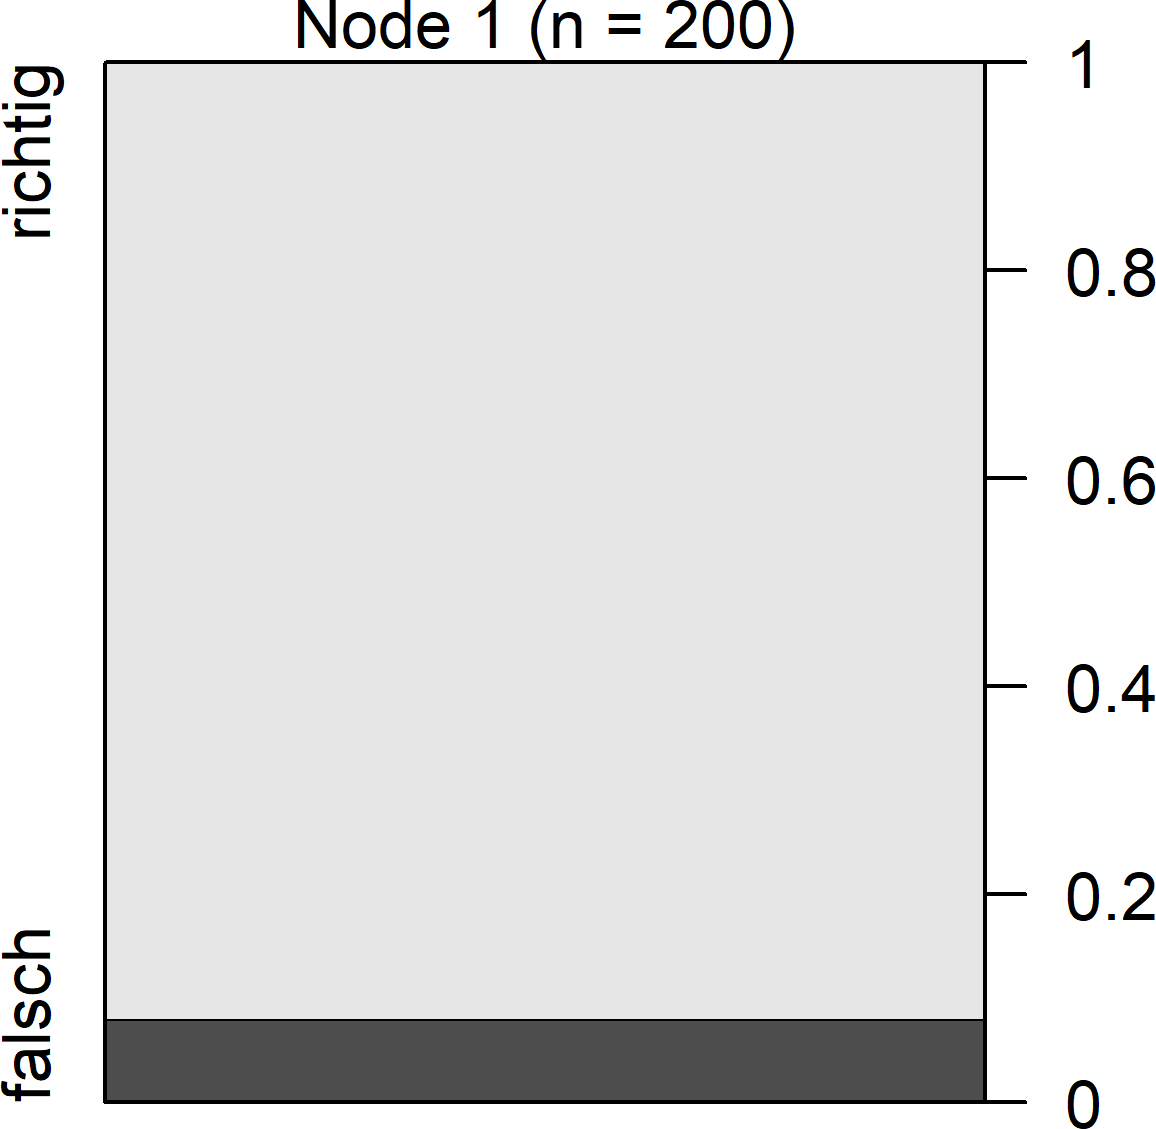
\includegraphics[scale=0.7]{CtreeGenitivDankKorr.png}
\caption{Conditional Inference Tree für die Korrektheit der Genitivrektion bei \dank}
\label{pic:AnhCtreeKorrGenitivrDank}
\end{figure}

\begin{figure}
\centering
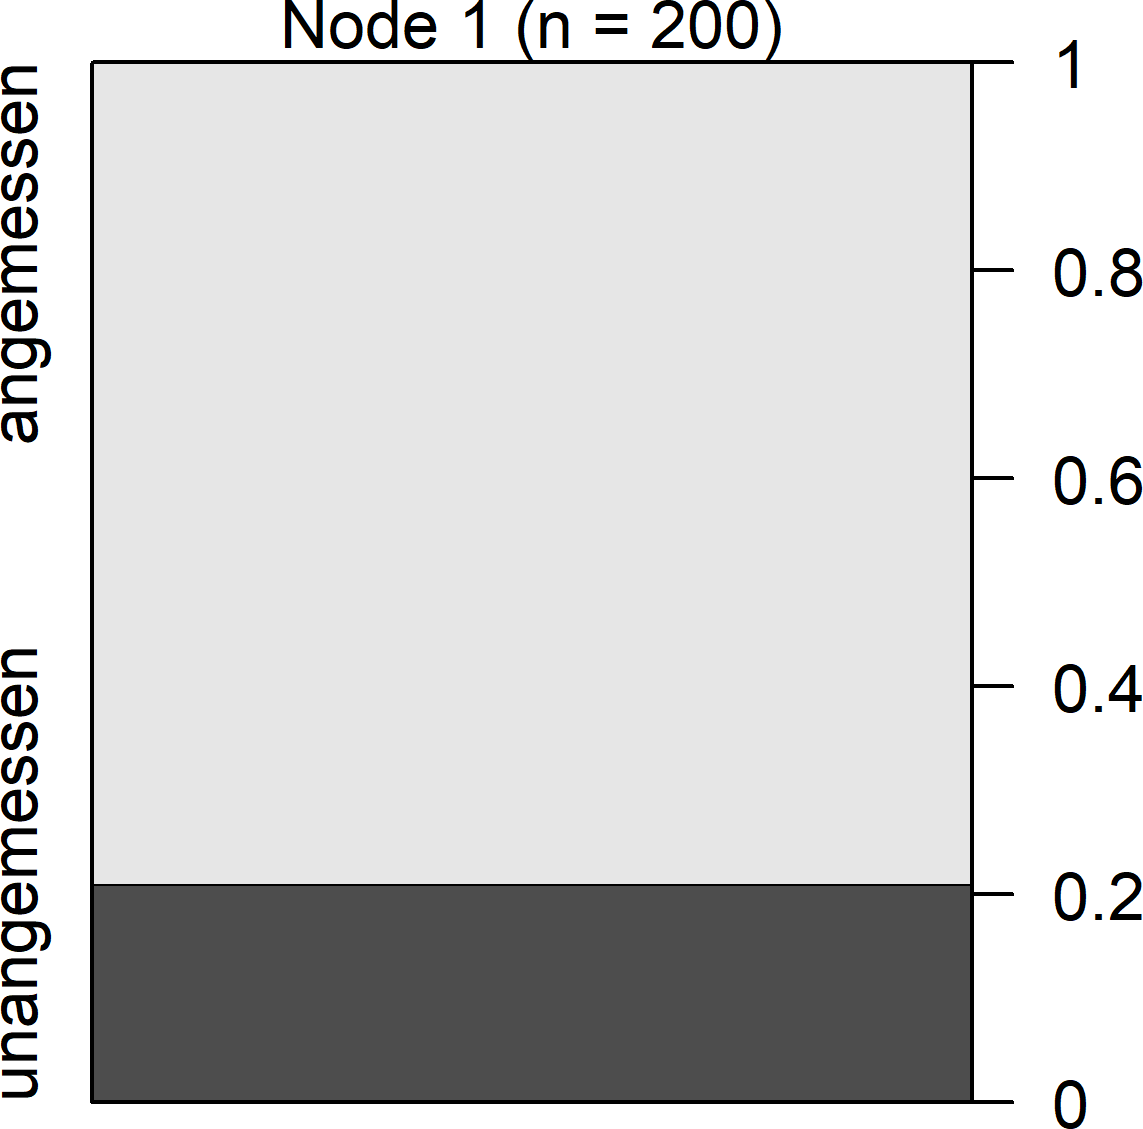
\includegraphics[scale=0.7]{CtreeGenitivDankAng.png}
\caption{Conditional Inference Tree für die Angemessenheit der Genitivrektion bei \dank}
\label{pic:AnhCtreeAngGenitivrDank}
\end{figure}

\begin{figure}
\centering
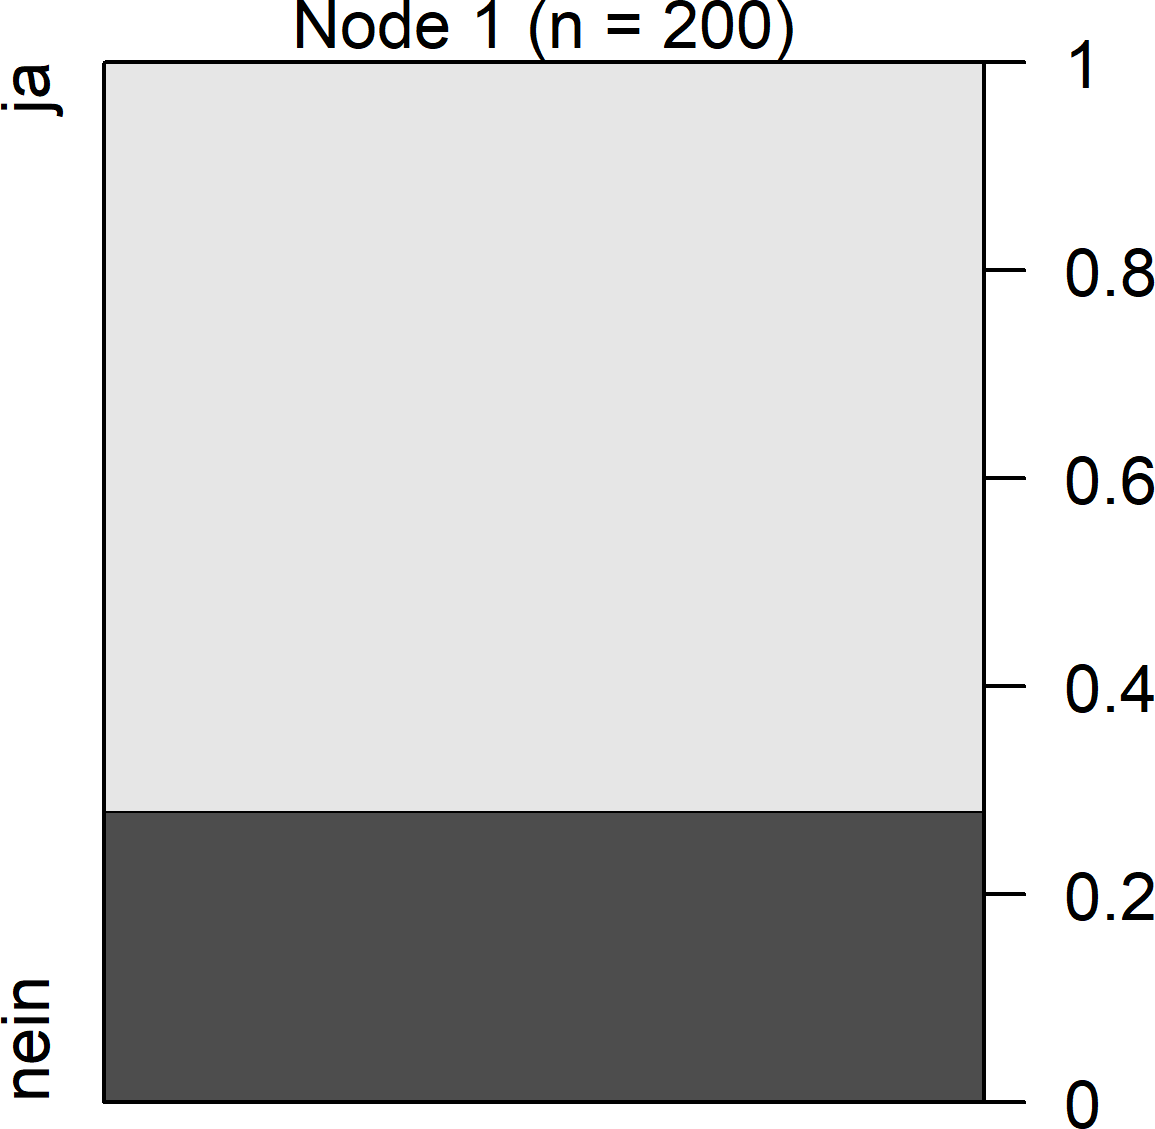
\includegraphics[scale=0.7]{CtreeGenitivDankVerw.png}
\caption{Conditional Inference Tree für die Angaben zur eigenen Verwendung der Genitivrektion bei \dank}
\label{pic:AnhCtreeVerwGenitivrDank}
\end{figure}

\begin{figure}
\centering
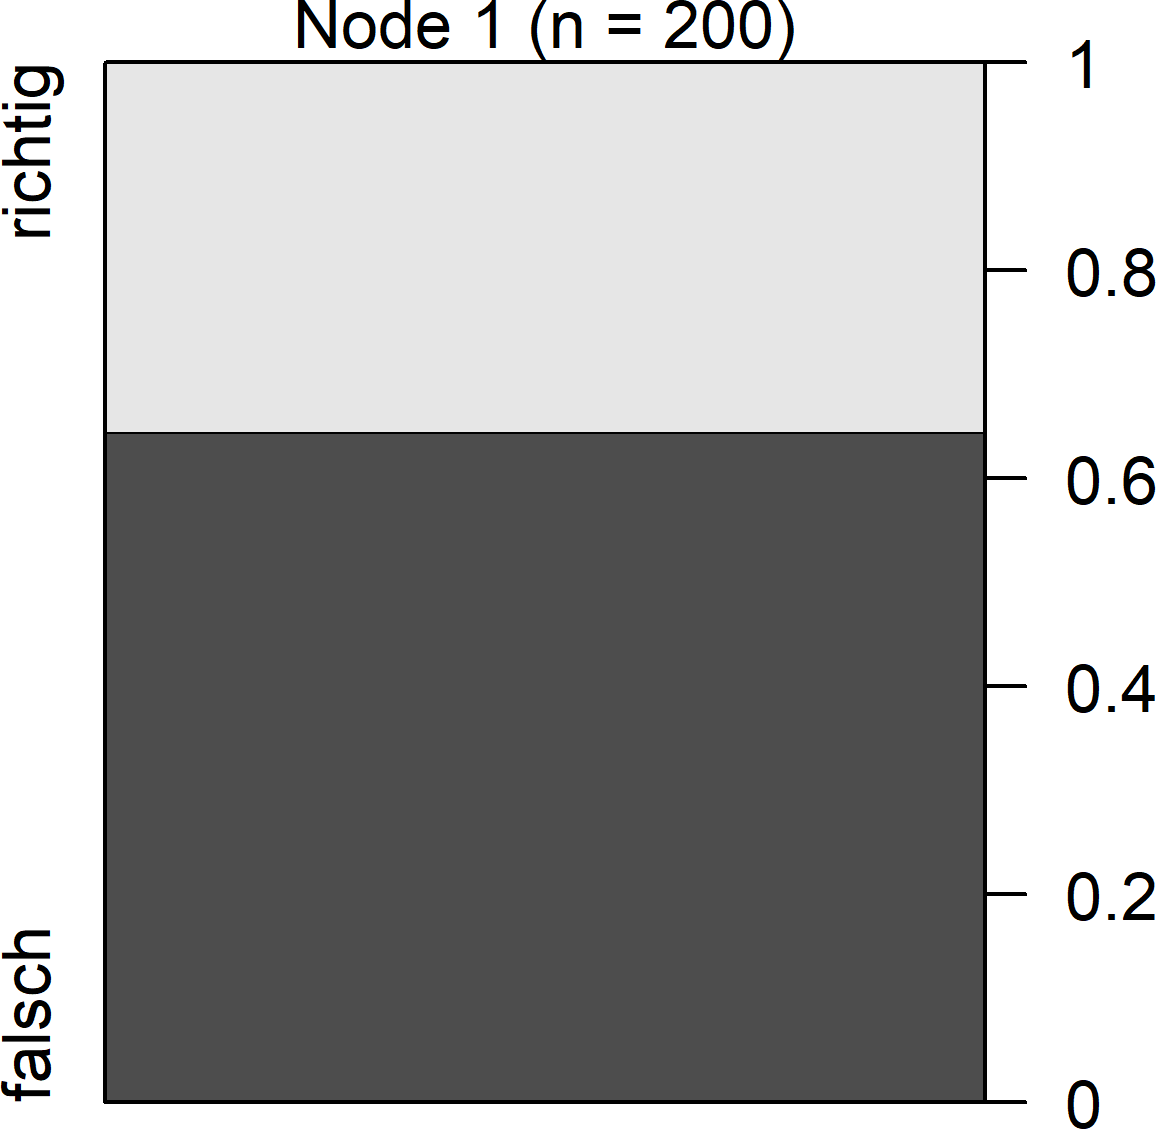
\includegraphics[scale=0.7]{CtreeGenitivGegenueberKorr.png}
\caption{Conditional Inference Tree für die Korrektheit der Genitivrektion bei \gegenueber}
\label{pic:AnhCtreeKorrGenitivrGegenueber}
\end{figure}

\begin{figure}
\centering
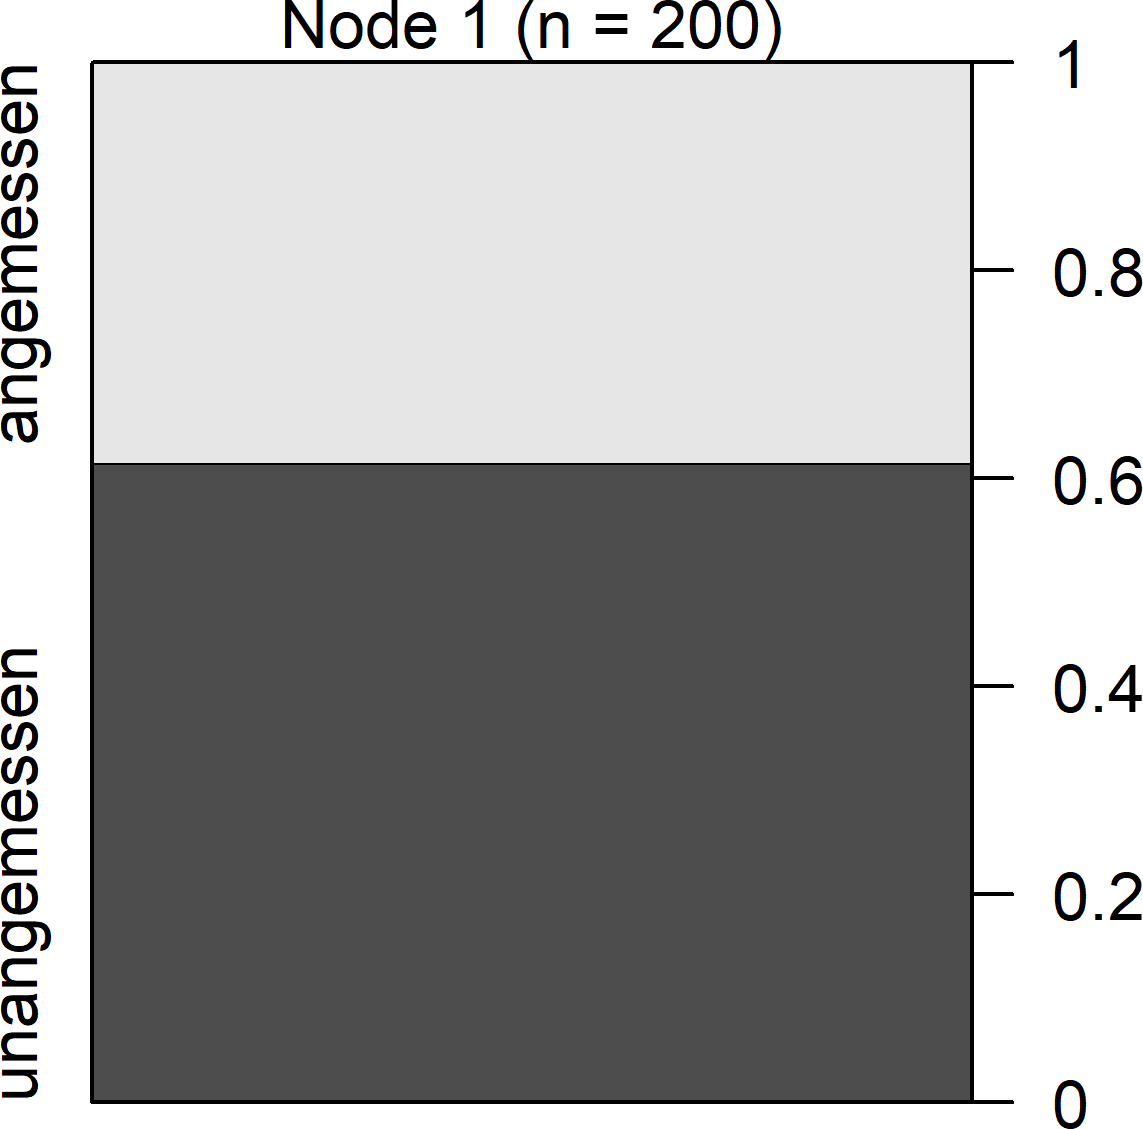
\includegraphics[scale=0.7]{CtreeGenitivGegenueberAng.png}
\caption{Conditional Inference Tree für die Angemessenheit der Genitivrektion bei \gegenueber}
\label{pic:AnhCtreeAngGenitivrGegenueber}
\end{figure}

\begin{figure}
\centering
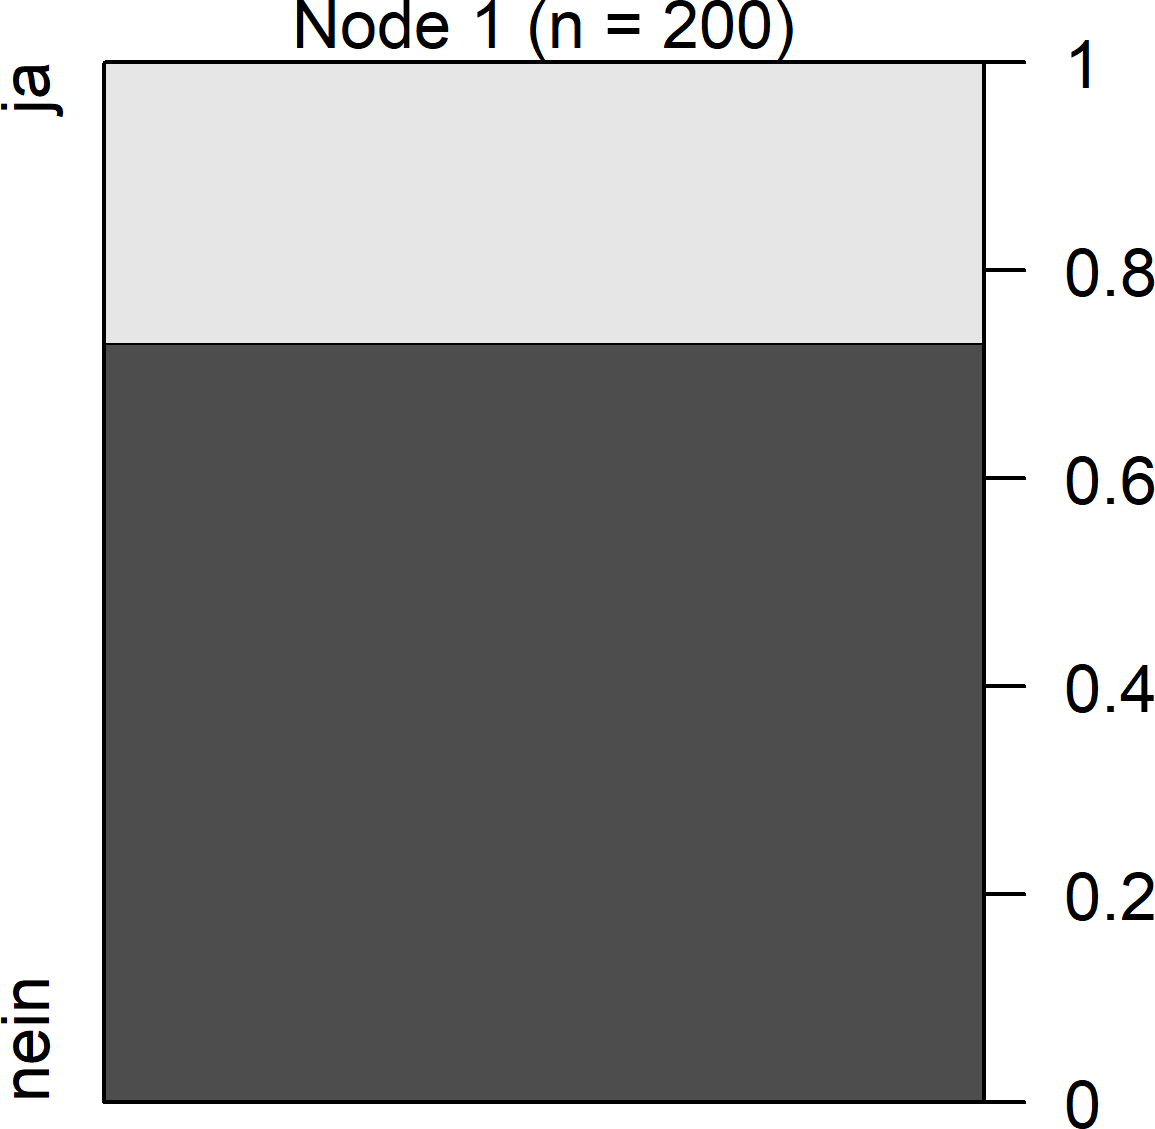
\includegraphics[scale=0.7]{CtreeGenitivGegenueberVerw.png}
\caption{Conditional Inference Tree für die Angaben zur eigenen Verwendung der Genitivrektion bei \gegenueber}
\label{pic:AnhCtreeVerwGenitivrGegenueber}
\end{figure}

\section*{Handbuch für die Kodierung der Begründungen im Akzeptabilitätstest}
\label{Anh:HandbuchBegr}
% Please add the following required packages to your document preamble:
% \usepackage{lscape}
% \usepackage{longtable}
% Note: It may be necessary to compile the document several times to get a multi-page table to line up properly
\begin{longtable}{|l|l|l|l|l|l|}
\hline
%\multicolumn{6}{|l|}{\textbf{Handbuch für die Kategorisierung der Begründungen aus dem Akzeptabilitätstest}}                                                                                                                                                                                                                                                                                                                                                                                                                                                                                                                                                                                                                                                                                                   \\ \hline
%\endhead
%
\multicolumn{6}{|l|}{\begin{tabular}[c]{@{}l@{}}Allgemeines: Als Kodierungseinheit dient immer der komplette Eintrag einer befragten Person. Die \\ Kodierungseinheiten können doppelt kodiert werden, d.h., sie müssen nicht einer Kategorie zugeordnet werden, \\ in die sie ausschließlich passen. Als Code dienen immer nur die jeweils untersten Kategorieenebenen, d.\,h., eine \\ Einheit wird z.\,B. nur der Kategorie \glqq schlecht/unschön\grqq{} zugeordnet, nicht zusätzlich den darüberliegenden \\ Kategorien \glqq nicht ästhetisch\grqq{} und \glqq Ästhetik\grqq. Bei Einordnung in die Kategorie \glqq nicht entscheidbar\grqq{} ist eine \\ Anmerkung hilfreich, warum keine Entscheidung möglich ist.\end{tabular}}                                                                                                                     \\ \hline
\multicolumn{5}{|l|}{\textbf{Kategorien}}                                                            & \textbf{Beschreibung und Beispiele}                                                                                                                                                                                                                                                                                                                                                                                                                                                                                                                                                                                                                                                                                   \\ \hline
\endfirsthead
%
\hline
\multicolumn{5}{|l|}{\textbf{Kategorien}}      & \textbf{Beschreibung und Beispiele}                    \\ \hline
\endhead
%
     & \multicolumn{4}{l|}{\textbf{Korrektheit}}                                                     & \begin{tabular}[c]{@{}l@{}}Begründungen, die sich auf die Inkorrektheit \\ (oder Korrektheit) der Form beziehen; die Codes \\ \glqq falsch\grqq{} und \glqq richtig\grqq{} können in manchen Fällen   \\ zusammen vergeben werden, wenn gesagt wird, dass \\ eine Variante in einem Kontext falsch, in einem \\ anderen aber richtig ist\end{tabular}                                                                                                                                                                                                                                                                                                                                                                      \\ \hline
     & \textbf{}          & \multicolumn{3}{l|}{falsch}                                              & Bsp.: \textit{\glqq gegenüber\grqq{} fordert Dativ                                                                                                                                                                                                                                                                                                                                                                                                                                                                                                                                                                                                                                                                      } \\ \hline
     & \textbf{}          & \multicolumn{3}{l|}{richtig}                                             & \begin{tabular}[c]{@{}l@{}}Meist einschränkend\\      \\ Bsp.: \textit{Es ist meines Wissens nach beides richtig,}\\ \textit{aber der Genitiv klingt besser}\end{tabular}                                                                                                                                                                                                                                                                                                                                                                                                                                                                                                                                                                            \\ \hline
          & \multicolumn{4}{l|}{\textbf{Herleitung}}                                                      & \begin{tabular}[c]{@{}l@{}}Begründungen, die etwa die Herkunft einer Variante \\ anführen\\ \\ Bsp. 1: \textit{Es heißt auch \glqq Dank ihm... dank ihr,,,\grqq{} deshalb} \\ \textit{müsste der Dativ auch bei Dank dem Sachbearbeiter} \\ \textit{heißen, oder aber konsequent \glqq Dank seiner\grqq, was kein} \\ \textit{Mensch annähme.}\\ Bsp. 2: \textit{gegenüber von wem?}\end{tabular}                                                                                                                                                                                                                                                                                                                                                                        \\ \hline
               & \multicolumn{4}{l|}{\textbf{Zweifel}}                                                         & \begin{tabular}[c]{@{}l@{}}Äußerung   von Unsicherheit in Bezug auf die Varianten\\      \\ Bsp.: \textit{muss es nicht Dativ sein?} \end{tabular}                                                                                                                                                                                                                                                                                                                                                                                                                                                                                               \\ \hline
                    & \multicolumn{4}{l|}{\textbf{Gleichgültigkeit}}                                                & \begin{tabular}[c]{@{}l@{}}Wahrscheinlich selten, da ja begründet werden soll, \\ warum eine Variante als unangemessen eingestuft wurde.\end{tabular}                                                                                                                                                                                                                                                                                                                                                                                                                                                                                                                                                   \\ \hline
                         & \multicolumn{4}{l|}{\textbf{eigener Sprachgebrauch}}                                              & \begin{tabular}[c]{@{}l@{}}Aussagen, die   die Variante zum eigenen Sprachgebrauch \\ in Beziehung setzen\end{tabular}                                                                                                                                                                                                                                                                                                                                                                                                                                                                                                                                                                                  \\ \hline
     & \textbf{}          & \multicolumn{3}{l|}{entspricht eigenem Gebrauch nicht}                   & Bsp.:   \textit{Würde dem verwenden                                                                                                                                                                                                                                                                                                                                                                                                                                                                                                                                                                                                                                                                            } \\ \hline
     & \textbf{}          & \multicolumn{3}{l|}{entspricht eigenem Gebrauch}                         &                                                                                                                                                                                                                                                                                                                                                                                                                                                                                                                                                                                                                                                                                                         \\ \hline
     & \multicolumn{4}{l|}{\textbf{Sprachgefühl}}                                                    & \begin{tabular}[c]{@{}l@{}}Antworten,   in denen das eigene Sprachgefühl/\\die Intuition als Grund angeführt wird\end{tabular}                                                                                                                                                                                                                                                                                                                                                                                                                                                                                                                                                                         \\ \hline
\newpage          & \multicolumn{4}{l|}{\textbf{Sprachwandel}}                                                    &                                                                                                                                                                                                                                                                                                                                                                                                                                                                                                                                                                                                                                                                                                         \\ \hline
     & \textbf{}          & \multicolumn{3}{l|}{Sprachverfall}                                       & \begin{tabular}[c]{@{}l@{}}Variante wird abgelehnt, da sie für einen zu\\ verhindernden Sprachwandel steht.\\      \\ Bsp.: \textit{Der Dativ ist dem Genitiv sein Tod}\end{tabular}                                                                                                                                                                                                                                                                                                                                                                                                                                                                                                                            \\ \hline
     & \textbf{}          & \multicolumn{3}{l|}{natürlicher Wandel}                                  & \begin{tabular}[c]{@{}l@{}}Bsp.: \textit{Während des Vortrags ist heute}\\ \textit{gebräuchlich}\end{tabular}                                                                                                                                                                                                                                                                                                                                                                                                                                                                                                                                                                                 \\ \hline
     & \multicolumn{4}{l|}{\textbf{Formalität}}                                                        & \begin{tabular}[c]{@{}l@{}}Äußerungen, die die Unangemessenheit mit der\\ Zugehörigkeit zu einem Register begründen.\\   Hier wird zwischen zwei Argumentationsweisen\\ unterschieden: \\ 1. Die Variante selbst wirkt informell/formell.\\ Bsp.: \textit{hört sich zu formell an}\\ 2. Der Kontext fordert eine bestimmte Formalität. \\ Bsp.: \textit{Zu förmlich in der Alltagssprache}\\      \\ Hier geht es nicht um die Begründungen mit einem\\ bestimmten Äußerungsmedium. Mediale Begründungen\\ und formalitätsbezogene Begründungen   überschneiden\\ sich aber häufig und lassen sich schwer trennen.\\ Im   Zweifelsfall sollten daher beide Codes \\ vergeben werden.\end{tabular}                          \\ \hline
     & \textbf{}          & \multicolumn{3}{l|}{Variante wirkt informell}                                & \begin{tabular}[c]{@{}l@{}}Bsp.:   \textit{Nicht förmlich genug}\end{tabular}                                                                                                                                                                                                                                                                                                                                                                                                                                                                                                                                                                                                                                                                                                                                                                                                                                                                                                                                                                                                                                                                                                                                                                                                                                                                                        \\ \hline
     & \textbf{}          & \multicolumn{3}{l|}{Variante wirkt formell}                                    & \textit{zu förmlich}                                                                                                                                                                                                                                                                                                                                                                                                                                                                                                                                                                                                                                                                                                         \\ \hline
     & \textbf{}          & \multicolumn{3}{l|}{Kontext fordert Informalität}                                   &                                                                                                                                                                                                                                                                                                                                                                                                                                                                                                                                                                                                                                                                                                         \\ \hline
     & \textbf{}          & \multicolumn{3}{l|}{Kontext fordert Formalität}                                     & \begin{tabular}[c]{@{}l@{}}Bsp.:   \textit{Förmliche Briefe sollten auf korrekten Gebrauch} \\ \textit{der Grammatik achten.}\end{tabular}                                                                                                                                                                                                                                                                                                                                                                                                                                                                                                                                                                                \\ \hline
     & \multicolumn{4}{l|}{\textbf{Medium}}                                                          & \begin{tabular}[c]{@{}l@{}}Hier geht es nur um eine Zuordnung der Variante zu \\einem Medium. Wie bei Formalität   wird auch hier zwischen\\ zwei Argumentationen unterschieden: \\ 1. Die Variante wird mit einem bestimmten Medium\\ assoziiert.\\ 2. Das Medium fordert eine bestimmte Variante. \\ Es kann sein, dass beide Interpretationen anwendbar\\ sind, wie in diesem   Beispiel: \\ Bsp.: \textit{Eigentlich müsste es Genitiv sein, ist aber in}  \\ \textit{einem Gespräch in Ordnung}\\      \\ Mediale Begründungen und formalitätsbezogene\\Begründungen überschneiden sich   aber häufig und \\lassen sich schwer trennen. Im Zweifelsfall sollten\\ daher beide Codes vergeben werden.\end{tabular} \\ \hline
     & \textbf{}          & \multicolumn{3}{l|}{Variante wirkt schriftlich}                          &  \\ \hline
     & \textbf{}          & \multicolumn{3}{l|}{Variante wirkt mündlich}                             &                                                                                                                                                                                                                                                                                                                                                                                                                                                                                                                                                                                                                                                                                                         \\ \hline
     & \textbf{}          & \multicolumn{3}{l|}{Kontext fordert typisch   schriftliche Formen}       &                                                                                                                                                                                                                                                                                                                                                                                                                                                                                                                                                                                                                                                                                                         \\ \hline
     & \textbf{}          & \multicolumn{3}{l|}{Kontext fordert typisch   mündliche Formen}          &                                                                                                                                                                                                                                                                                                                                                                                                                                                                                                                                                                                                                                                                                                         \\ \hline
     & \multicolumn{4}{l|}{\textbf{Varietät}}                                                        & \begin{tabular}[c]{@{}l@{}}Hier geht es um   Zuordnungen der Variante zu einer \\ bestimmten Varietät. Wie bei Formalität und   Medium \\ wird auch hier zwischen zwei Argumentationen\\ unterschieden: \\ 1. Die Variante wird mit einer bestimmten Varietät\\ assoziiert.\\ 2. Es liegt eine Varietät vor, zu der die Variante nicht\\ passt/passt.  \\ Es kann sein, dass beide Interpretationen anwendbar\\ sind\end{tabular}                                                                                                                                                                                                                                                                                 \\ \hline
     & \textbf{}          & \multicolumn{3}{l|}{Variante wirkt   umgangs-/alltagssprachlich}         & \begin{tabular}[c]{@{}l@{}}Bsp.   1: \textit{\glqq wegen dem\grqq{} ist umgangssprachlich}\\ Bsp. 2: \textit{\glqq wegen des Kontos\grqq{} ist richtig. in}\\ \textit{Umgangssprache ok, nicht in einem förmlichen Brief.}\\ (muss zusätzlich in \glqq Formalität>Kontext fordert \\ Formalität\grqq{} kodiert werden)\end{tabular}                                                                                                                                                                                                                                                                                                                                                                                                                                  \\ \hline
     & \textbf{}          & \multicolumn{3}{l|}{Variante wirkt   regionalsprachlich/dialektal}       &                                                                                                                                                                                                                                                                                                                                                                                                                                                                                                                                                                                                                                                                                                         \\ \hline
     & \textbf{}          & \multicolumn{3}{l|}{Variante wirkt   standardsprachlich}                 &                                                                                                                                                                                                                                                                                                                                                                                                                                                                                                                                                                                                                                                                                                         \\ \hline
     & \textbf{}          & \multicolumn{3}{l|}{Kontext fordert   Umgangs-/Alltagssprache}           & \begin{tabular}[c]{@{}l@{}}Bsp.:   \textit{Zu förmlich in der Alltagssprache }(muss zusätzlich \\ in \glqq Variante wirkt formell\grqq{} kodiert   werden)\end{tabular}                                                                                                                                                                                                                                                                                                                                                                                                                                                                                                                                                     \\ \hline
     & \textbf{}          & \multicolumn{3}{l|}{Kontext fordert   Regionalsprache/Dialekt}           &                                                                                                                                                                                                                                                                                                                                                                                                                                                                                                                                                                                                                                                                                                         \\ \hline
     & \textbf{}          & \multicolumn{3}{l|}{Kontext fordert   Standardsprache}                   &                                                                                                                                                                                                                                                                                                                                                                                                                                                                                                                                                                                                                                                                                                         \\ \hline
     & \multicolumn{4}{l|}{\textbf{Ästhetik}}                                                        & \begin{tabular}[c]{@{}l@{}}Einstufung als unangemessen wird mit dem Klang \\ einer Variante etc. begründet. Hier geht es zum einen \\ darum, ob eine Form als schön/unschön empfunden \\ wird, zum anderen   darum, ob Varianten als \\ auffällig empfunden werden.\end{tabular}                                                                                                                                                                                                                                                                                                                                                                                                                        \\ \hline
     & \textbf{}          & \multicolumn{3}{l|}{unlogisch}                                           & \begin{tabular}[c]{@{}l@{}}neu   hinzugekommen \\      \\ Bsp.: \textit{falsch, macht keinen Sinn}\end{tabular}                                                                                                                                                                                                                                                                                                                                                                                                                                                                                                                                                                                                  \\ \hline
     & \textbf{}          & \multicolumn{3}{l|}{überflüssig/unnötig}                                 & neu   hinzugekommen                                                                                                                                                                                                                                                                                                                                                                                                                                                                                                                                                                                                                                                                                     \\ \hline
     & \textbf{}          & \multicolumn{3}{l|}{simpel}                                              &                                                                                                                                                                                                                                                                                                                                                                                                                                                                                                                                                                                                                                                                                                         \\ \hline
     & \textbf{}          & \multicolumn{3}{l|}{auffällig/ungewohnt}                                 &                                                                                                                                                                                                                                                                                                                                                                                                                                                                                                                                                                                                                                                                                                         \\ \hline
     & \textbf{}          & \multicolumn{3}{l|}{unauffällig/normal}                                  &                                                                                                                                                                                                                                                                                                                                                                                                                                                                                                                                                                                                                                                                                                         \\ \hline
     & \textbf{}          & \multicolumn{3}{l|}{ästhetisch}                                          &                                                                                                                                                                                                                                                                                                                                                                                                                                                                                                                                                                                                                                                                                                         \\ \hline
     & \textbf{}          &            & \multicolumn{2}{l|}{gut/schön}                              &                                                                                                                                                                                                                                                                                                                                                                                                                                                                                                                                                                                                                                                                                                         \\ \hline
     & \textbf{}          &            & \multicolumn{2}{l|}{elegant/gehoben}                        &                                                                                                                                                                                                                                                                                                                                                                                                                                                                                                                                                                                                                                                                                                         \\ \hline
     & \textbf{}          & \multicolumn{3}{l|}{nicht   ästhetisch}                                  &                                                                                                                                                                                                                                                                                                                                                                                                                                                                                                                                                                                                                                                                                                         \\ \hline
     & \textbf{}          &            & \multicolumn{2}{l|}{schlecht/unschön}                       & \begin{tabular}[c]{@{}l@{}}Bsp.:   \textit{besser: dem Schaffner }(in Bezug auf des \\ Schaffners zeigt diese Äußerung, dass die Genitivvariante\\ als weniger gut empfunden wird.)\end{tabular}                                                                                                                                                                                                                                                                                                                                                                                                                                                                                                               \\ \hline
     & \textbf{}          &            & \multicolumn{2}{l|}{umständlich}                            &                                                                                                                                                                                                                                                                                                                                                                                                                                                                                                                                                                                                                                                                                                         \\ \hline
     & \textbf{}          &            & \multicolumn{2}{l|}{gestelzt/abgehoben/überkorrekt}         &                                                                                                                                                                                                                                                                                                                                                                                                                                                                                                                                                                                                                                                                                                         \\ \hline
     & \textbf{}          &            & \multicolumn{2}{l|}{plump/schlampig}                        &                                                                                                                                                                                                                                                                                                                                                                                                                                                                                                                                                                                                                                                                                                         \\ \hline
     & \multicolumn{4}{l|}{\textbf{Bedeutung und  Verständlichkeit}}                                & \begin{tabular}[c]{@{}l@{}}Begründungen mit der Verständlichkeit oder der \\ Bedeutung einer Variante\\      \\ Bsp.: \textit{grammatikalisch falsch, außer man will eine} \\ \textit{Ortsangabe ausdrücken}.\end{tabular}                                                                                                                                                                                                                                                                                                                                                                                                                                                                                             \\ \hline
          & \multicolumn{4}{l|}{\textbf{Personentypus}}                                          & \begin{tabular}[c]{@{}l@{}}Begründungen, die sich auf mit der Variante verbundene \\ Personeneigenschaften beziehen.\end{tabular}                                                                                                                                                                                                                                                                                                                                                                                                                                                                                                                                                                     \\ \hline
     & \textbf{}          & \multicolumn{3}{l|}{Vertrautheit}                                        & Nähe der Kommunikationspartner zueinander                                                                                                                                                                                                                                                                                                                                                                                                                                                                                                                                                                                                                                                               \\ \hline
     & \textbf{}          &            & \multicolumn{2}{l|}{Fremdheit/Distanz}                      & wirkt fremd/passt nur in distanzierten Kontexten                                                                                                                                                                                                                                                                                                                                                                                                                                                                                                                                                                                                                                                        \\ \hline
     & \textbf{}          &            & \multicolumn{2}{l|}{Vertrautheit/Nähe}                      & wirkt vertraut/passt nur in privaten Kontexten                                                                                                                                                                                                                                                                                                                                                                                                                                                                                                                                                                                                                                                          \\ \hline
     &                    & \multicolumn{3}{l|}{Charakter}                                           & \begin{tabular}[c]{@{}l@{}}Begründungen,   die sich auf charakterliche Eigenschaften \\ der Personen beziehen, die eine   solche Variante äußern\end{tabular}                                                                                                                                                                                                                                                                                                                                                                                                                                                                                                                                           \\ \hline
     &                    &            & \multicolumn{2}{l|}{präzise/professionell/vertrauenswürdig} & \begin{tabular}[c]{@{}l@{}}Variante   wirkt sorgfältig, professionell, überlegt, \\ kompetent etc.\end{tabular}                                                                                                                                                                                                                                                                                                                                                                                                                                                                                                                                                                                         \\ \hline
     &                    &            & \multicolumn{2}{l|}{vornehm/altmodisch}                     & wirkt   vornehm/altmodisch                                                                                                                                                                                                                                                                                                                                                                                                                                                                                                                                                                                                                                                                              \\ \hline
     &                    &            & \multicolumn{2}{l|}{unsympathisch}                          & Bsp.:   \textit{Ungebildete Leute finde ich nicht sehr sympatisch.}                                                                                                                                                                                                                                                                                                                                                                                                                                                                                                                                                                                                                                              \\ \hline
     &                    &            & \multicolumn{2}{l|}{sympathisch/mir ähnlich}                & wirkt   sympathisch                                                                                                                                                                                                                                                                                                                                                                                                                                                                                                                                                                                                                                                                                     \\ \hline
     &                    &            & \multicolumn{2}{l|}{besserwisserisch}                       & wirkt   besserwisserisch                                                                                                                                                                                                                                                                                                                                                                                                                                                                                                                                                                                                                                                                                \\ \hline
     &                    &            & \multicolumn{2}{l|}{unfreundlich}                           & wirkt   unfreundlich                                                                                                                                                                                                                                                                                                                                                                                                                                                                                                                                                                                                                                                                                    \\ \hline
     &                    &            & \multicolumn{2}{l|}{streng/seriös}                          & wirkt   streng/seriös                                                                                                                                                                                                                                                                                                                                                                                                                                                                                                                                                                                                                                                                                   \\ \hline
     &                    &            & \multicolumn{2}{l|}{locker/unprätentiös}                    & wirkt   locker                                                                                                                                                                                                                                                                                                                                                                                                                                                                                                                                                                                                                                                                                          \\ \hline
     &                    &            & \multicolumn{2}{l|}{abgehoben/arrogant}                     & wirkt   arrogant                                                                                                                                                                                                                                                                                                                                                                                                                                                                                                                                                                                                                                                                                        \\ \hline
     &                    &            & \multicolumn{2}{l|}{pedantisch/verkrampft}                  & wirkt   verkrampft                                                                                                                                                                                                                                                                                                                                                                                                                                                                                                                                                                                                                                                                                      \\ \hline
     &                    &            & \multicolumn{2}{l|}{nachlässig/schlampig}                   & wirkt   schlampig/ungenau                                                                                                                                                                                                                                                                                                                                                                                                                                                                                                                                                                                                                                                                               \\ \hline
     &                    & \multicolumn{3}{l|}{bestimmte   Gruppe}                                  & \begin{tabular}[c]{@{}l@{}}Zuordnung der   Variante zu einer bestimmten \\ Gruppe\end{tabular}                                                                                                                                                                                                                                                                                                                                                                                                                                                                                                                                                                                                          \\ \hline
     &                    &            & \multicolumn{2}{l|}{ArbeiterInnen}                          &                                                                                                                                                                                                                                                                                                                                                                                                                                                                                                                                                                                                                                                                                                         \\ \hline
     &                    &            & \multicolumn{2}{l|}{Unterschicht}                           &                                                                                                                                                                                                                                                                                                                                                                                                                                                                                                                                                                                                                                                                                                         \\ \hline
     &                    &            & \multicolumn{2}{l|}{Technische Berufe}                      &                                                                                                                                                                                                                                                                                                                                                                                                                                                                                                                                                                                                                                                                                                         \\ \hline
     &                    &            & \multicolumn{2}{l|}{AkademikerInnen/GymnasiastInnen}        &                                                                                                                                                                                                                                                                                                                                                                                                                                                                                                                                                                                                                                                                                                         \\ \hline
     &                    &            & \multicolumn{2}{l|}{Beruflich Erfolgreiche}                 &                                                                                                                                                                                                                                                                                                                                                                                                                                                                                                                                                                                                                                                                                                         \\ \hline
     &                    &            & \multicolumn{2}{l|}{Bourgeoisie}                            &                                                                                                                                                                                                                                                                                                                                                                                                                                                                                                                                                                                                                                                                                                         \\ \hline
     &                    &            & \multicolumn{2}{l|}{Ältere   Leute}                         &                                                                                                                                                                                                                                                                                                                                                                                                                                                                                                                                                                                                                                                                                                         \\ \hline
     &                    &            & \multicolumn{2}{l|}{Kinder}                                 &                                                                                                                                                                                                                                                                                                                                                                                                                                                                                                                                                                                                                                                                                                         \\ \hline
     &                    &            & \multicolumn{2}{l|}{Junge Leute}                            &                                                                                                                                                                                                                                                                                                                                                                                                                                                                                                                                                                                                                                                                                                         \\ \hline
     &                    & \multicolumn{3}{l|}{Bildung}                                             & \begin{tabular}[c]{@{}l@{}}Variante wird   als Zeichen hoher oder niedriger \\ Bildung gesehen\end{tabular}                                                                                                                                                                                                                                                                                                                                                                                                                                                                                                                                                                                             \\ \hline
     &                    &            & \multicolumn{2}{l|}{niedrige Bildung}                       &                                                                                                                                                                                                                                                                                                                                                                                                                                                                                                                                                                                                                                                                                                         \\ \hline
     &                    &            & \multicolumn{2}{l|}{hohe Bildung}                           &                                                                                                                                                                                                                                                                                                                                                                                                                                                                                                                                                                                                                                                                                                         \\ \hline
     &                    & \multicolumn{3}{l|}{Sprachkompetenz}                                     & \begin{tabular}[c]{@{}l@{}}Variante   wird als Zeichen hoher oder niedriger \\ Sprachkompetenz gesehen.\end{tabular}                                                                                                                                                                                                                                                                                                                                                                                                                                                                                                                                                                                    \\ \hline
     &                    &            & \multicolumn{2}{l|}{hohe Sprachkompetenz}                   &                                                                                                                                                                                                                                                                                                                                                                                                                                                                                                                                                                                                                                                                                                         \\ \hline
     &                    &            & \multicolumn{2}{l|}{mangelnde Sprachkompetenz}              &                                                                                                                                                                                                                                                                                                                                                                                                                                                                                                                                                                                                                                                                                                         \\ \hline
     & \multicolumn{4}{l|}{\textbf{nur Vorschlag oder Benennung}}               & \begin{tabular}[c]{@{}l@{}}In vielen Äußerungen findet sich zwar ein Hinweis \\ darauf, was im Beispiel als unangemessen empfunden \\ wurde, oder es wird ein Alternativvorschlag gemacht, \\ eine Begründung fehlt jedoch.\\      \\ Bsp. 1: \textit{Dativ nötig}\\ Bsp. 2: \textit{Genitiv statt Dativ}\\ Bsp. 3: \textit{Genitiv nicht verwendet}\end{tabular}                                                                                                                                                                                                                                                                                   \\ \hline
     & \multicolumn{4}{l|}{\textbf{nicht relevant/nicht   auf den Kasus bezogen}}                    & \begin{tabular}[c]{@{}l@{}}Begründungen, die zeigen, dass die Einstufung als \\ unangemessen nicht aufgrund des Kasus   vorgenommen \\ wurde und sich zum Beispiel auf den Ihnalt des Satzes \\ beziehen. Dieser Code wird nicht gemeinsam mit \\ anderen vergeben.\\ \\ Bsp.: \textit{Name des Sachbearbeiters fehlt}\end{tabular}                                                                                                                                                                                                                                                                                                                                                                           \\ \hline
     & \multicolumn{4}{l|}{\textbf{keine Angabe}}                                                    & \begin{tabular}[c]{@{}l@{}}Entweder expliziter Hinweis, dass nichts stört (Einträge \\ wie \textit{nichts} etc.) oder   Einträge wie \glqq--\grqq. \\ Dieser Code wird nur vergeben, wenn die ganze Aussage \\ weder einen Vorschlag,   noch eine Benennung der \\ störenden Form, noch eine Begründung erkennen lässt.\end{tabular}                                                                                                                                                                                                                                                                                                                                                                                      \\ \hline
     & \multicolumn{4}{l|}{\textbf{nicht entscheidbar}}                                              & \begin{tabular}[c]{@{}l@{}}Äußerungen, die keiner Kategorie eindeutig zugeordnet \\ werden können, weil nicht klar ist, worauf sie sich \\ beziehen\\      \\ Bsp.: \textit{Grammatik}\end{tabular}                                                                                                                                                                                                                                                                                                                                                                                                                                                                                                              \\ \hline
\end{longtable}

\section*{Ergebnisse des Produktionsexperiments}
% Please add the following required packages to your document preamble:
% \usepackage{multirow}
\begin{table}
\centering
\begin{tabular}{llrrr}
                                                                                           & \textit{\textbf{}} & \multicolumn{1}{l}{\textbf{Dativ}}                       & \multicolumn{1}{l}{\textbf{Genitiv}}                     & \multicolumn{1}{l}{\textbf{Sonstige}}                  \\ \hline
\multirow{5}{*}{\textbf{\begin{tabular}[c]{@{}l@{}}formeller\\ Lückentext\end{tabular}}}   & \textit{wegen}     & \begin{tabular}[c]{@{}r@{}}51\\ (12,85 \%)\end{tabular}  & \begin{tabular}[c]{@{}r@{}}345\\ (86,9 \%)\end{tabular}  & \begin{tabular}[c]{@{}r@{}}1\\ (0,25 \%)\end{tabular}  \\ \cline{2-5} 
                                                                                           & \textit{während}   & \begin{tabular}[c]{@{}r@{}}25\\ (6,3 \%)\end{tabular}    & \begin{tabular}[c]{@{}r@{}}371\\ (93,45 \%)\end{tabular} & \begin{tabular}[c]{@{}r@{}}1\\ (0,25 \%)\end{tabular}  \\ \cline{2-5} 
                                                                                           & \textit{dank}      & \begin{tabular}[c]{@{}r@{}}31\\ (7,81 \%)\end{tabular}   & \begin{tabular}[c]{@{}r@{}}364\\ (91,69 \%)\end{tabular} & \begin{tabular}[c]{@{}r@{}}2\\ (0,5 \%)\end{tabular}   \\ \cline{2-5} 
                                                                                           & \textit{gegenüber} & \begin{tabular}[c]{@{}r@{}}357\\ (89,92 \%)\end{tabular} & \begin{tabular}[c]{@{}r@{}}32\\ (8,06 \%)\end{tabular}   & \begin{tabular}[c]{@{}r@{}}8\\ (2,02 \%)\end{tabular}  \\ \cline{2-5} 
                                                                                           & \textit{seit}      & \begin{tabular}[c]{@{}r@{}}351\\ (88,41 \%)\end{tabular} & \begin{tabular}[c]{@{}r@{}}44\\ (11,08 \%)\end{tabular}  & \begin{tabular}[c]{@{}r@{}}2\\ (0,5 \%)\end{tabular}   \\ \hline
\multicolumn{5}{l}{\textbf{}}                                                                                                                                                                                                                                                                  \\ \hline
\multirow{5}{*}{\textbf{\begin{tabular}[c]{@{}l@{}}informeller\\ Lückentext\end{tabular}}} & \textit{wegen}     & \begin{tabular}[c]{@{}r@{}}114\\ (28,72 \%)\end{tabular} & \begin{tabular}[c]{@{}r@{}}278\\ (70,03 \%)\end{tabular} & \begin{tabular}[c]{@{}r@{}}5\\ (1,26 \%)\end{tabular}  \\ \cline{2-5} 
                                                                                           & \textit{während}   & \begin{tabular}[c]{@{}r@{}}73\\ (18,39 \%)\end{tabular}  & \begin{tabular}[c]{@{}r@{}}321\\ (80,86 \%)\end{tabular} & \begin{tabular}[c]{@{}r@{}}3\\ (0,76 \%)\end{tabular}  \\ \cline{2-5} 
                                                                                           & \textit{dank}      & \begin{tabular}[c]{@{}r@{}}66\\ (16,62 \%)\end{tabular}  & \begin{tabular}[c]{@{}r@{}}327\\ (82,37 \%)\end{tabular} & \begin{tabular}[c]{@{}r@{}}4\\ (1,01 \%)\end{tabular}  \\ \cline{2-5} 
                                                                                           & \textit{gegenüber} & \begin{tabular}[c]{@{}r@{}}350\\ (88,16 \%)\end{tabular} & \begin{tabular}[c]{@{}r@{}}37\\ (9,32 \%)\end{tabular}   & \begin{tabular}[c]{@{}r@{}}10\\ (2,52 \%)\end{tabular} \\ \cline{2-5} 
                                                                                           & \textit{seit}      & \begin{tabular}[c]{@{}r@{}}373\\ (93,95 \%)\end{tabular} & \begin{tabular}[c]{@{}r@{}}23\\ (5,79 \%)\end{tabular}   & \begin{tabular}[c]{@{}r@{}}1\\ (0,25 \%)\end{tabular}  \\
\end{tabular}
\caption{Ergebnisse des Produktionsexperiments (n=397)}
\label{table:AnhProd}
\end{table}

% Please add the following required packages to your document preamble:
% \usepackage{multirow}
\begin{table}
\centering
\begin{tabular}{llrr|rr}
\multicolumn{6}{l}{\textit{\textbf{wegen}}}                                                                                                                                                                                                                                               \\ \hline
                                                                                  &           & \multicolumn{2}{c}{\begin{tabular}[c]{@{}c@{}}\textbf{Ss+}\\ (n=344)\end{tabular}} & \multicolumn{2}{|c}{\begin{tabular}[c]{@{}c@{}}\textbf{Ss--}\\ (n=53)\end{tabular}} \\ \hline
\multirow{3}{*}{\begin{tabular}[c]{@{}l@{}}formeller \\ Lückentext\end{tabular}}  & Dativ     & 40                                        & (11,63 \%)                                      & 11                                         & (20,75 \%)                                         \\ %\cline{2-6} 
                                                                                  & Genitiv   & 304                                       & (88,37 \%)                                      & 41                                         & (77,36 \%)                                         \\ %\cline{2-6} 
                                                                                  & Sonstiges  & 0                                         & (0 \%)                                          & 1                                          & (1,89 \%)                                          \\ \hline
\textbf{}                                                                         & \textbf{} & \multicolumn{2}{c}{\begin{tabular}[c]{@{}c@{}}\textbf{Ss+}\\ (n=344)\end{tabular}} & \multicolumn{2}{|c}{\begin{tabular}[c]{@{}c@{}}\textbf{Ss--}\\ (n=53)\end{tabular}}  \\ \hline
\multirow{3}{*}{\begin{tabular}[c]{@{}l@{}}informeller\\ Lückentext\end{tabular}} & Dativ     & 89                                        & (25,87 \%)                                      & 25                                         & (47,17 \%)                                         \\ %\cline{2-6} 
                                                                                  & Genitiv   & 250                                       & (72,67 \%)                                       & 28                                         & (52,83 \%)                                         \\ %\cline{2-6} 
                                                                                  & Sonstiges  & 5                                         & (1,45 \%)                                       & 0                                          & (0 \%)                                          \\ \hline
\end{tabular}
\caption{Kasuswahl bei \wegen{} im formellen und im informellen Lückentext nach Sprachsicherheit}
\label{table:AnhErgProdWegenNachSs}
\end{table}
% Please add the following required packages to your document preamble:
% \usepackage{multirow}
\begin{table}
\centering
\begin{tabular}{llrr|rr}
\multicolumn{6}{l}{\textit{\textbf{während}}}                                                                                                                                                                                                                                                  \\ \hline
                                                                                  &           & \multicolumn{2}{c}{\begin{tabular}[c]{@{}c@{}}\textbf{Ss+}\\ (n=344)\end{tabular}} & \multicolumn{2}{|c}{\begin{tabular}[c]{@{}c@{}}\textbf{Ss--}\\ (n=53)\end{tabular}} \\ \hline
\multirow{3}{*}{\begin{tabular}[c]{@{}l@{}}formeller \\ Lückentext\end{tabular}}  & Dativ     & 19                                         & (5,52 \%)                                         & 6                                           & (11,32 \%)                                          \\ %\cline{2-6} 
                                                                                  & Genitiv   & 324                                        & (94,19 \%)                                        & 47                                          & (88,68 \%)                                          \\ %\cline{2-6} 
                                                                                  & Sonstiges  & 1                                          & (0,29 \%)                                         & 0                                           & (0 \%)                                              \\ \hline
\textbf{}                                                                         & \textbf{} & \multicolumn{2}{c}{\begin{tabular}[c]{@{}c@{}}\textbf{hohe}\\ \textbf{Sprachsicherheit}\\ (n=344)\end{tabular}} & \multicolumn{2}{|c}{\begin{tabular}[c]{@{}c@{}}\textbf{geringe}\\ \textbf{Sprachsicherheit}\\ (n=53)\end{tabular}}  \\ \hline
\multirow{3}{*}{\begin{tabular}[c]{@{}l@{}}informeller\\ Lückentext\end{tabular}} & Dativ     & 57                                         & (16,57 \%)                                        & 16                                          & (30,19 \%)                                          \\ %\cline{2-6} 
                                                                                  & Genitiv   & 285                                        & (82,85 \%)                                        & 36                                          & (67,92 \%)                                          \\ %\cline{2-6} 
                                                                                  & Sonstiges  & 2                                          & (0,58 \%)                                         & 1                                           & (1,89 \%)                                           \\ \hline
\end{tabular}
\caption{Kasuswahl bei \waehrend{} im formellen und im informellen Lückentext nach Sprachsicherheit}
\label{table:AnhErgProdWaehrendNachSs}
\end{table}
% Please add the following required packages to your document preamble:
% \usepackage{multirow}
\begin{table}
\centering
\begin{tabular}{llrr|rr}
\multicolumn{6}{l}{\textit{\textbf{dank}}}                                                                                                                                                                                                                                                     \\ \hline
                                                                                  &           & \multicolumn{2}{c}{\begin{tabular}[c]{@{}c@{}}\textbf{Ss+}\\ (n=344)\end{tabular}} & \multicolumn{2}{|c}{\begin{tabular}[c]{@{}c@{}}\textbf{Ss--}\\ (n=53)\end{tabular}} \\ \hline
\multirow{3}{*}{\begin{tabular}[c]{@{}l@{}}formeller \\ Lückentext\end{tabular}}  & Dativ     & 29                                         & (8,43 \%)                                         & 2                                           & (3,77 \%)                                           \\ %\cline{2-6} 
                                                                                  & Genitiv   & 314                                        & (91,28 \%)                                        & 50                                          & (94,34 \%)                                          \\ %\cline{2-6} 
                                                                                  & Sonstiges  & 1                                          & (0,29 \%)                                         & 1                                           & (1,89 \%)                                           \\ \hline
\textbf{}                                                                         & \textbf{} & \multicolumn{2}{c}{\begin{tabular}[c]{@{}c@{}}\textbf{Ss+}\\ (n=344)\end{tabular}} & \multicolumn{2}{|c}{\begin{tabular}[c]{@{}c@{}}\textbf{Ss--}\\ (n=53)\end{tabular}}  \\ \hline
\multirow{3}{*}{\begin{tabular}[c]{@{}l@{}}informeller\\ Lückentext\end{tabular}} & Dativ     & 57                                         & (16,57 \%)                                        & 9                                           & (16,98 \%)                                          \\ %\cline{2-6} 
                                                                                  & Genitiv   & 285                                        & (82,85 \%)                                        & 42                                          & (79,25 \%)                                          \\ %\cline{2-6} 
                                                                                  & Sonstiges  & 2                                          & (0,58 \%)                                         & 2                                           & (3,77 \%)                                           \\ \hline
\end{tabular}
\caption{Kasuswahl bei \dank{} im formellen und im informellen Lückentext nach Sprachsicherheit}
\label{table:AnhErgProdDankNachSs}
\end{table}
% Please add the following required packages to your document preamble:
% \usepackage{multirow}
\begin{table}
\centering
\begin{tabular}{llrr|rr}
\multicolumn{6}{l}{\textit{\textbf{gegenüber}}}                                                                                                                                                                                                                                                \\ \hline
                                                                                  &           & \multicolumn{2}{c}{\begin{tabular}[c]{@{}c@{}}\textbf{Ss+}\\ (n=344)\end{tabular}} & \multicolumn{2}{|c}{\begin{tabular}[c]{@{}c@{}}\textbf{Ss--}\\ (n=53)\end{tabular}} \\ \hline
\multirow{3}{*}{\begin{tabular}[c]{@{}l@{}}formeller \\ Lückentext\end{tabular}}  & Dativ     & 310                                        & (90,12 \%)                                        & 47                                          & (88,68 \%)                                          \\ %\cline{2-6} 
                                                                                  & Genitiv   & 27                                         & (7,85 \%)                                         & 5                                           & (9,43 \%)                                           \\ %\cline{2-6} 
                                                                                  & Sonstiges  & 7                                          & (2,03 \%)                                         & 1                                           & (1,89 \%)                                           \\ \hline
\textbf{}                                                                         & \textbf{} & \multicolumn{2}{c}{\begin{tabular}[c]{@{}c@{}}\textbf{Ss+}\\ (n=344)\end{tabular}} & \multicolumn{2}{|c}{\begin{tabular}[c]{@{}c@{}}\textbf{Ss--}\\ (n=53)\end{tabular}}  \\ \hline
\multirow{3}{*}{\begin{tabular}[c]{@{}l@{}}informeller\\ Lückentext\end{tabular}} & Dativ     & 307                                        & (89,24 \%)                                        & 43                                          & (81,13 \%)                                          \\ %\cline{2-6} 
                                                                                  & Genitiv   & 30                                         & (8,72 \%)                                         & 7                                           & (13,21 \%)                                          \\ %\cline{2-6} 
                                                                                  & Sonstiges  & 7                                          & (2,03 \%)                                         & 3                                           & (5,66 \%)                                           \\ \hline
\end{tabular}
\caption{Kasuswahl bei \gegenueber{} im formellen und im informellen Lückentext nach Sprachsicherheit}
\label{table:AnhErgProdGegenueberNachSs}
\end{table}
% Please add the following required packages to your document preamble:
% \usepackage{multirow}
\begin{table}
\centering
\begin{tabular}{llrr|rr}
\multicolumn{6}{l}{\textit{\textbf{seit}}}                                                                                                                                                                                                                                                     \\ \hline
                                                                                  &           & \multicolumn{2}{c}{\begin{tabular}[c]{@{}c@{}}\textbf{Ss+}\\ (n=344)\end{tabular}} & \multicolumn{2}{|c}{\begin{tabular}[c]{@{}c@{}}\textbf{Ss--}\\ (n=53)\end{tabular}} \\ \hline
\multirow{3}{*}{\begin{tabular}[c]{@{}l@{}}formeller \\ Lückentext\end{tabular}}  & Dativ     & 309                                        & (89,83 \%)                                        & 42                                          & (79,25 \%)                                          \\ %\cline{2-6} 
                                                                                  & Genitiv   & 34                                         & (9,88 \%)                                         & 10                                          & (18,87 \%)                                          \\ %\cline{2-6} 
                                                                                  & Sonstiges  & 1                                          & (0,29 \%)                                         & 1                                           & (1,89 \%)                                           \\ \hline
\textbf{}                                                                         & \textbf{} & \multicolumn{2}{c}{\begin{tabular}[c]{@{}c@{}}\textbf{Ss+}\\ (n=344)\end{tabular}} & \multicolumn{2}{|c}{\begin{tabular}[c]{@{}c@{}}\textbf{Ss--}\\ (n=53)\end{tabular}}  \\ \hline
\multirow{3}{*}{\begin{tabular}[c]{@{}l@{}}informeller\\ Lückentext\end{tabular}} & Dativ     & 322                                        & (93,6 \%)                                         & 51                                          & (96,23 \%)                                          \\ %\cline{2-6} 
                                                                                  & Genitiv   & 21                                         & (6,1 \%)                                          & 2                                           & (3,77 \%)                                           \\ %\cline{2-6} 
                                                                                  & Sonstiges  & 1                                          & (0,29 \%)                                         & 0                                           & (0 \%)                                              \\ \hline
\end{tabular}
\caption{Kasuswahl bei \object{seit} im formellen und im informellen Lückentext nach Sprachsicherheit}
\label{table:AnhErgProdSeitNachSs}
\end{table}
\begin{figure}
\centering
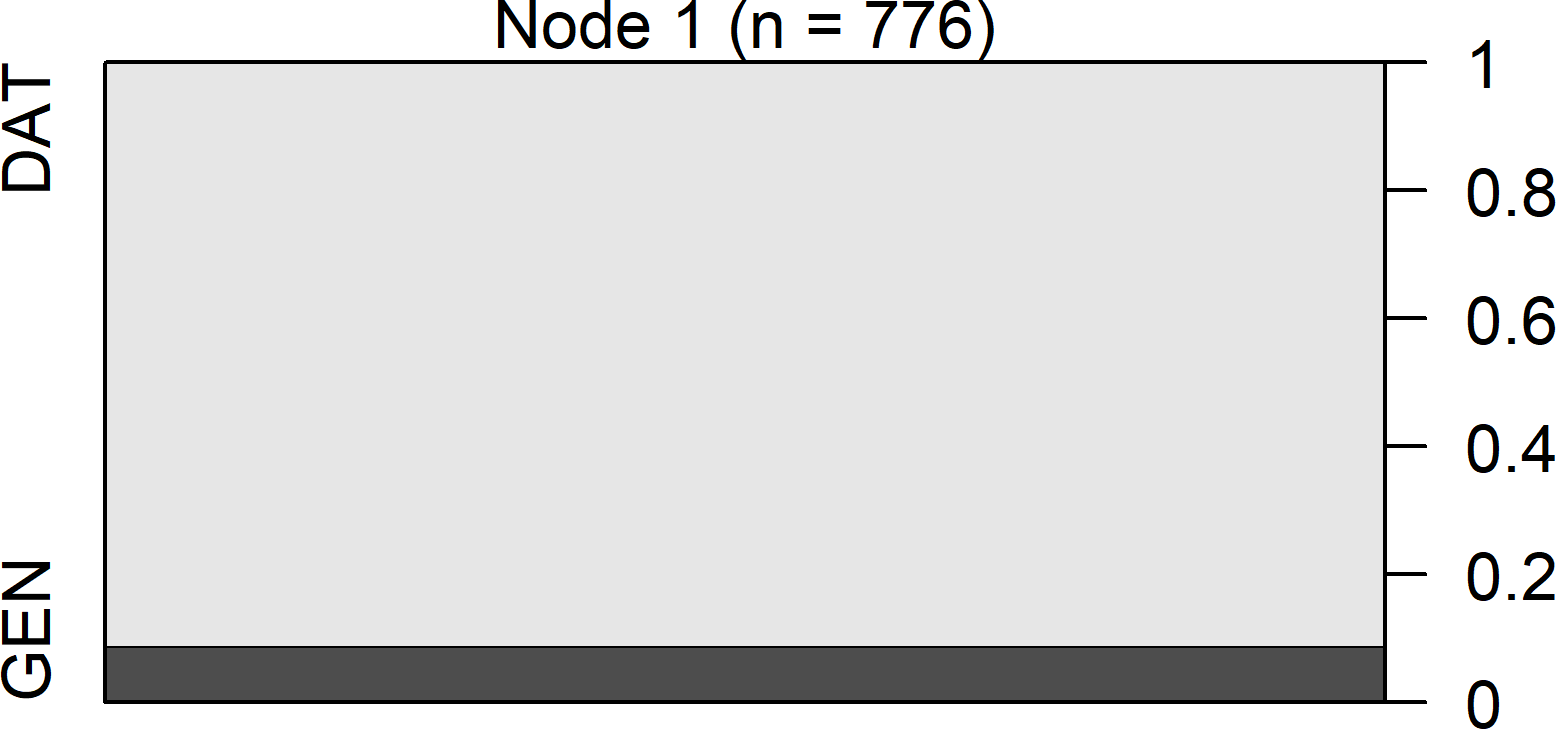
\includegraphics[scale=0.8]{CtreeProdgegenueber.png}
\caption{Conditional Inference Tree für die Kasuswahl bei \gegenueber}
\label{pic:AnhCtreeProdGegenueber}
\end{figure}
\begin{figure}
\centering
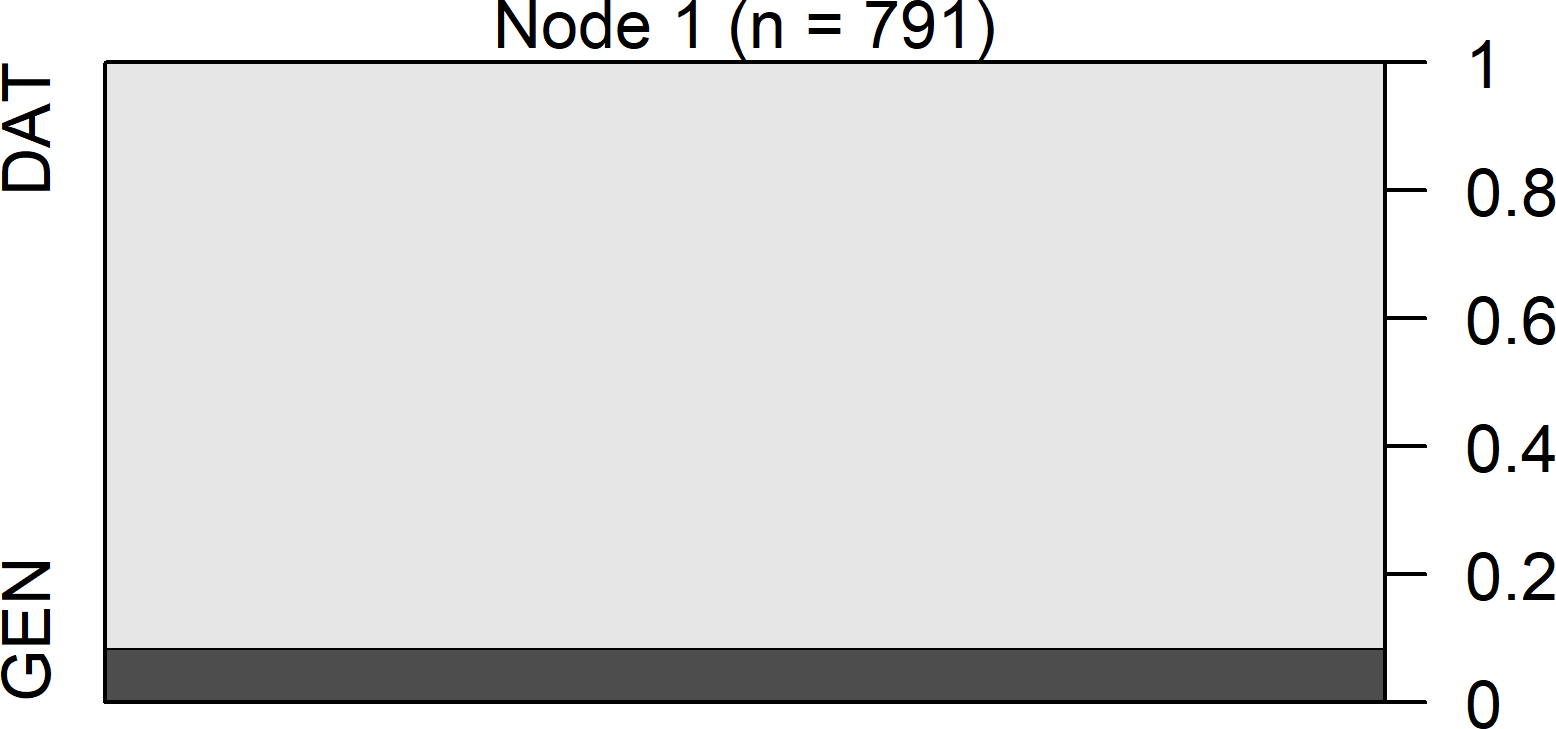
\includegraphics[scale=0.8]{CtreeProdseit.png}
\caption{Conditional Inference Tree für die Kasuswahl bei \object{seit}}
\label{pic:AnhCtreeProdSeit}
\end{figure}

\section*{Hinweise zum digitalen Anhang}
\label{sec:AnhHinweisDigitalerAnh}
\begin{itemize}
\item Der digitale Anhang ist unter folgender URL zugänglich:\\
https://osf.io/rmc5n/?view\_only=5d6e0a5c6bd84269a60193af9dc40175
\item Die R-Dateien finden sich im Ordner \glqq 1 R-Projekt\_Praepositionalkasus\_AV\grqq{}. 
Nach dem Download (den Ordner markieren und \glqq Download as zip\grqq{} wählen) sollten zunächst die erforderlichen Pakete geladen und ggf. installiert werden (s. Skript \glqq 00 Pakete installieren und laden\grqq). 
Als Encoding sollte utf-8 eingestellt werden.
Anschließend kann der Datensatz geladen werden (s. Skript \glqq 01 Daten laden und aufbereiten\grqq). 
Die Skripte für die Datenauswertung sind im Ordner \glqq R-Skripte\grqq{} zu finden. 
Alle Tabellen sind im Ordner \glqq logs\grqq{} gespeichert, alle Grafiken im Ordner \glqq graphs\grqq.
Im Ordner \glqq data\grqq{} finden sich der komplette Datensatz sowie Daten aus dem Pretest für die Itemanalyse der Likertskalen. 
\item Im Ordner \glqq 2 Kategorisierung in MAXQDA\_AV\grqq{} liegen die MAXQDA-Dateien mit den Kodierungen der Assoziationen und der Begründungen für die Einstufung als unangemessen im Akzeptabilitätstest. 
Für das Öffnen der Dateien ist das Programm MAXQDA erforderlich. 
Unter https://www.maxqda.de/software-inhaltsanalyse\#Demodownload lässt sich eine Testversion herunterladen. 
\end{itemize}
